\definecolor{verde_p}{rgb}{0.77,0.97,0.84}
\definecolor{amarillo_claro}{rgb}{1,1,0.90}

\chapter{Desarrollo del proyecto}

\section{Planteamiento inicial}

El desarrollo se ha llevado a cabo de manera modular. Se ha planteado el trabajo en bloques individuales para terminar comunicándolos por su respectiva vía.

Los objetivos descritos en la sección \ref{sec:refobj} sirven de guía para definir responsabilidades de cada módulo.

En la figura \ref{fig:diainteraccion} se puede observar el diagrama de interacciones entre los diferentes módulos

\begin{figure}[tb]
\centering
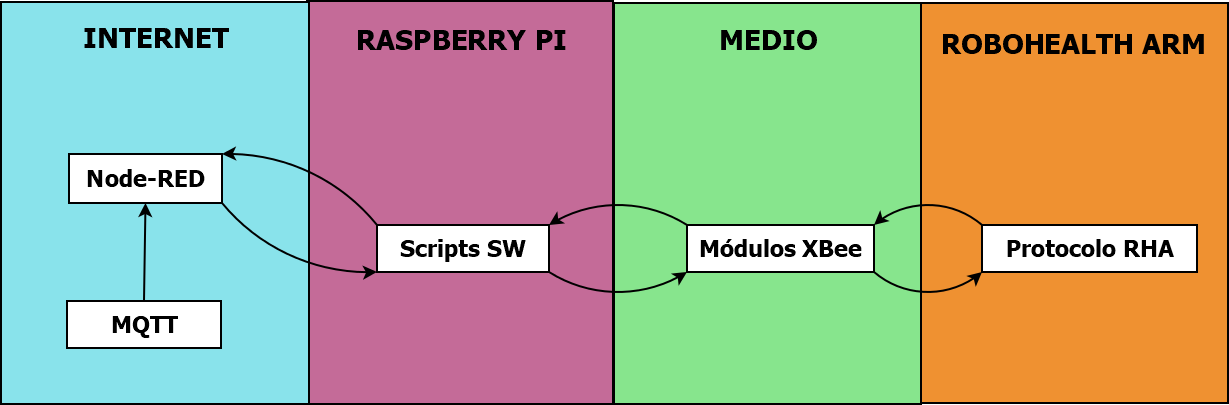
\includegraphics[width=1\textwidth]{figuras/DiaInteraccion.png}
\caption{Diagrama de interacción}
\label{fig:diainteraccion}
\end{figure}

Se establece una comunicación bidireccional en la que, por un lado, se envían comandos desde varias fuentes de mando y, por el otro, se reciben los mensajes periódicos de estado que envía el RoboHealth Arm.

Las fuentes de mando se emplazan en la red, desde donde se interactúa con el usuario. Una de ellas es Node-RED, la base de la red domótica y la otra es Mosquitto (MQTT), que diversifica el tipo de dispositivos desde los que se puede interactuar con el brazo.

La Raspberry Pi es el punto donde las órdenes enviadas desde la red toman forma en una salida serial.

Los módulos XBee se encargan de la transmisión inalámbrica de la información a través del medio\footnote{En la sección \ref{sec:radiofrec} se detalla el proceso del envío de ondas electromagnéticas a través del aire}.

Esta información es captada por el brazo robótico de acuerdo a un protocolo de comunicación prediseñado y actúa en consecuencia.

Haciendo una analogía con los diagramas de casos de uso propios del Lenguaje de Modelado Unificado (UML) en el campo del desarrollo software, a continuación (figura \ref{fig:diacasos}) se analizan las distintas acciones que puede efectuar el usuario y cómo debería reaccionar el sistema ante estas acciones. Nótese que se ha tomado al brazo robótico como un actor más dentro del sistema domótico.

\begin{figure}[tb]
\centering
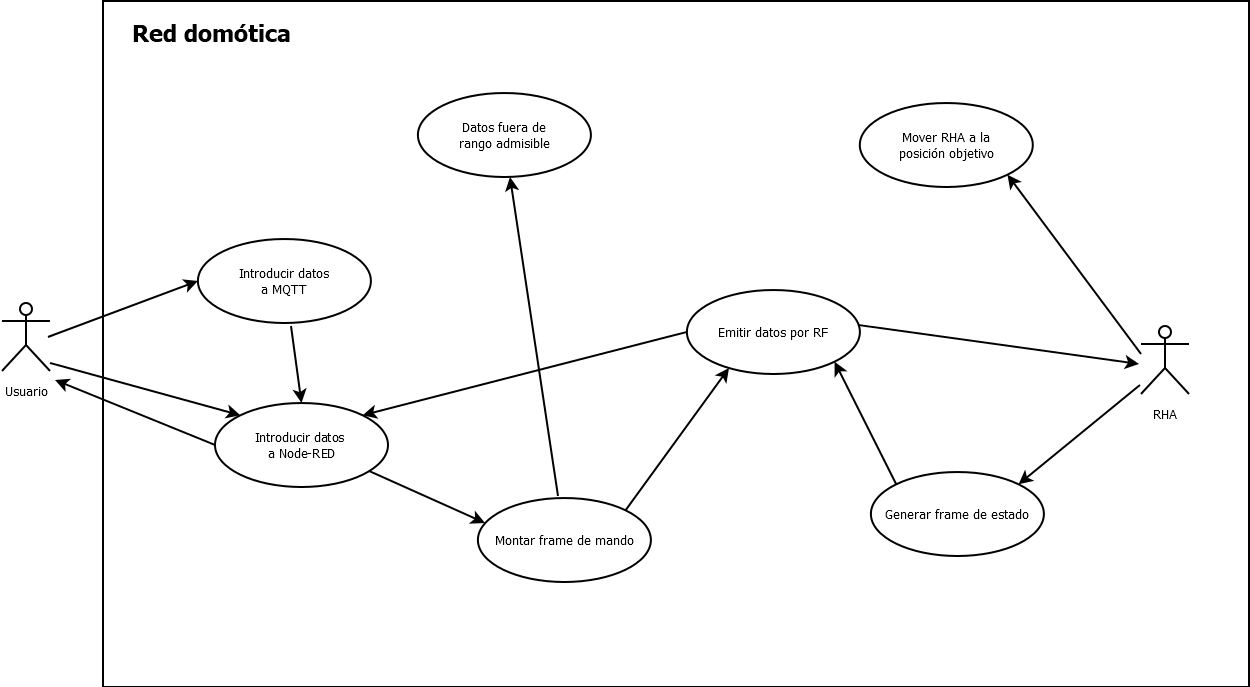
\includegraphics[width=1\textwidth]{figuras/DiaCasos.png}
\caption{Diagrama de casos de uso}
\label{fig:diacasos}
\end{figure}

Continuando con el uso de conceptos UML, en la imagen \ref{fig:diasecuencia} se puede observar la secuencia de acciones planificadas para el envío de información al brazo robótico.

\begin{figure}[tb]
\centering
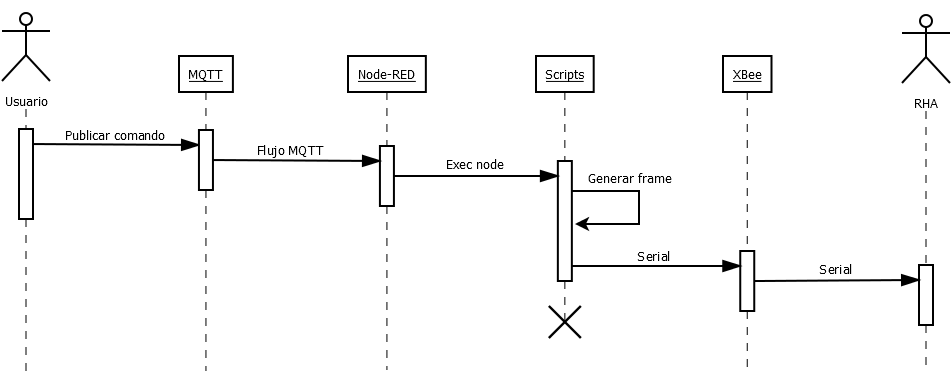
\includegraphics[width=1\textwidth]{figuras/DiaSecuencia.png}
\caption{Diagrama de Secuencia de envío}
\label{fig:diasecuencia}
\end{figure}

Con los objetivos y conceptos establecidos, se puede pasar al desarrollo siguiendo una metodología modular, como se ha indicado antes.

\section{Unidad de mando}

La base de las comunicaciones debe ser un ordenador. Las funciones de este ordenador o unidad de mando pasan por la coordinación de los diferentes elementos de la red domótica, incluyendo tanto el control de estos como la recepción de sus estados.

Es posible (y deseable) que ciertos elementos tengan otro control independiente a la red domótica. Así, por ejemplo, una persiana conectada a la red domótica podría ser accionada por el mismo ordenador sin obviar que el mecanismo podría accionarse a través de un pulsador. Esto hace necesaria la monitorización de la mayor parte posible de elementos. Podría darse el caso de que, incluso, la acción de ciertos elementos fuera mecánica en complementación a la acción de naturaleza electrica, imposibilitando cualquier integración de estos métodos alternativos de accionamiento en la red domótica. 

La unidad de mando debe encargarse de igual manera de la interacción con el usuario, aportando una interfaz.

Los requisitos de un sistema domótico no son especialmente exigentes en cuanto a la capacidad de procesamiento, por lo que características como un tamaño contenido o un bajo coste se valoran positivamente en la elección del ordenador0
.
En este contexto, se hace uso de la popular Raspberry Pi 3 Model B (figura \ref{fig:RPi3}) para el cometido descrito.

\subsection{Rasberry Pi 3 Model B}

La Raspberry Pi 3 Model B es uno de los más actuales modelos\footnote{Sólo se encuentra la Raspberry Pi 3 Model B+ con una fecha de lanzamiento posterior} de la tercera generación de este popular micro-ordenador de bajo coste. Si se miran sus especificaciones, se puede observar que, corriendo a través de una CPU Broadcom BCM2837 de 64 bits a 1.2GHz, posee:

\begin{itemize}
\item 1GB de memoria RAM
\item Conexión LAN inalámbrica y módulo Bluetooth integrados
\item Puerto Ethernet
\item 40 pines de entrada/salida (GPIO)
\item 4 puertos USB 2.0
\item Salida stereo de 4 polos
\item Conector HDMI
\item Puerto de cámara CSI
\item Puerto de display DSI
\item Puerto microSD
\item Puerto microUSB
\end{itemize}

Se puede observar el layout de estos componentes sobre la placa en la figura \ref{fig:RPilayout}.

\begin{figure}[tb]
\centering
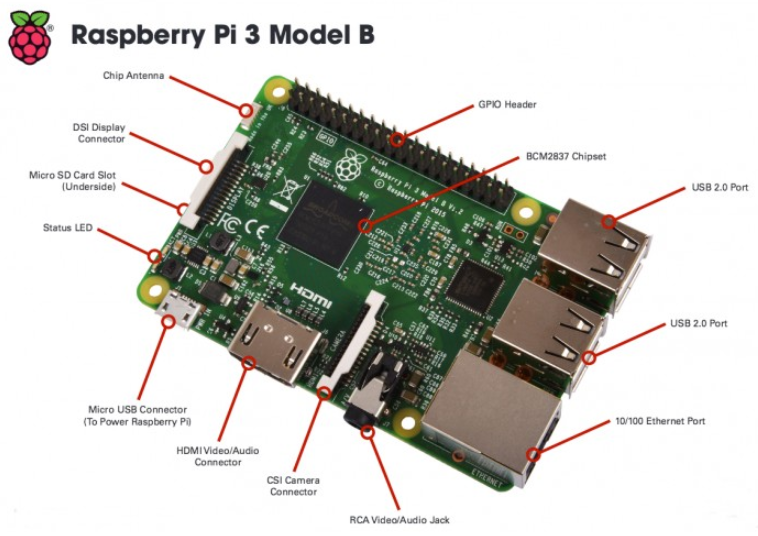
\includegraphics[width=0.75\textwidth]{figuras/RPiLayout.png}
\caption{Layout de puertos de la Raspberry Pi}
\label{fig:RPilayout}
\end{figure}

El puerto microUSB tiene la función de alimentar al ordenador. Se debe conectar una alimentación de 5 voltios a 2.5 amperios. Podría funcionar con una fuente de menos potencia pero podría ser que no soportara la inclusión de ciertos periféricos.

El puerto microSD sirve de alojamiento para la memoria ROM de la Raspberry. A través de este puerto, se carga el sistema operativo y se utiliza la memoria libre como almacenamiento interno.

\subsubsection{Raspbian OS}

Raspbian OS es el sistema operativo utilizado en la Raspberry Pi del laboratorio (figura \ref{fig:raspbian}). Se trata de una distribución no oficial basada en Debian adaptada a las especificaciones de la placa computadora Raspberry Pi. Debian está basado en el sistema GNU/Linux y, por tanto, se habla de software libre. El software, con sus características y actualizaciones, es desarrollado por la comunidad.

\begin{figure}[tb]
\centering
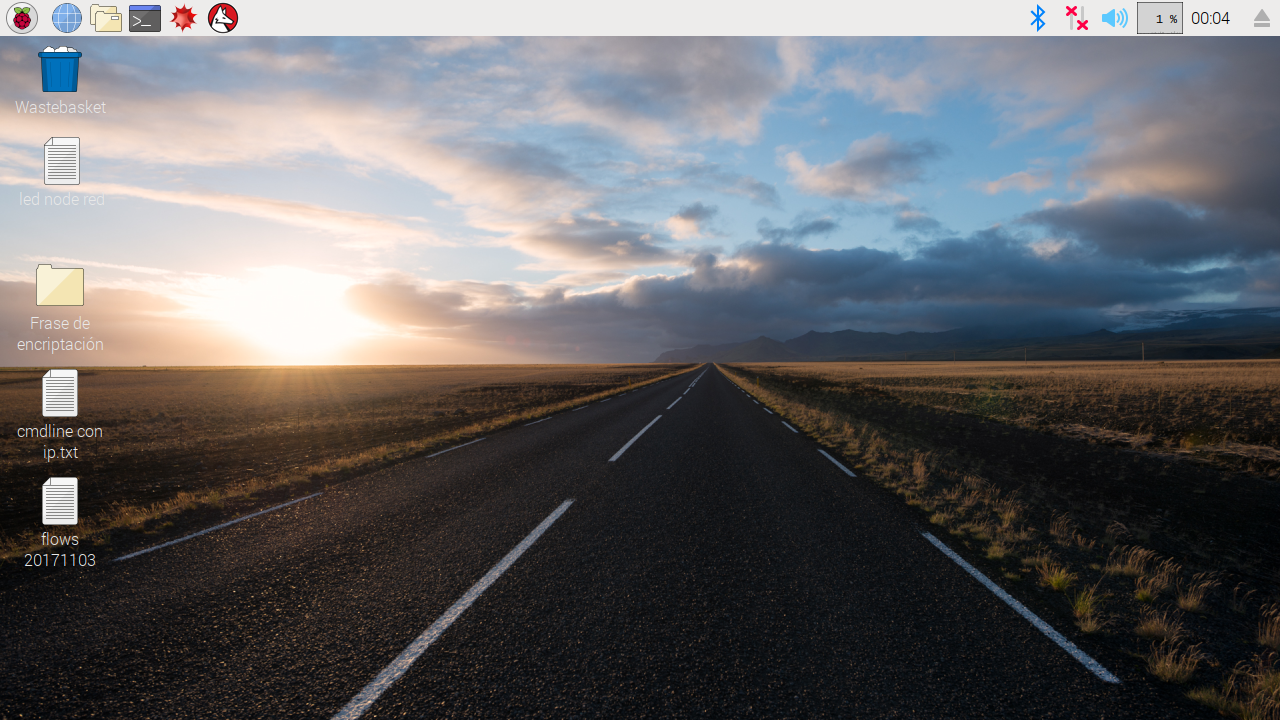
\includegraphics[width=0.7\textwidth]{figuras/Raspbian.png}
\caption{Escritorio de Raspbian}
\label{fig:raspbian}
\end{figure}

Entre otras funcionalidades, destaca el poder configurar la Raspberry de manera sencilla a través del menú \textit{raspy-config}

En el Anexo \ref{anexo:raspbian} se encuentran las instrucciones para obtener Raspbian 9.1 (Stretch) instalado en la Raspberry. Esta es la última distribución estable a día de hoy.

\subsubsection{Comunicación con otros ordenadores}

% Configuración de la visualización del código SW
\lstset{backgroundcolor=\color{verde_p}, language=bash, breaklines=true, basicstyle=\footnotesize, xleftmargin=25pt, framesep=8pt, numbersep=15pt}

A la hora de trabajar con la Raspberry instalada, no es usual que sea deseable la instalación de periféricos de entrada y salida para interactuar con ella. Es por esto por lo que se recurre a una conexión SSH para trabajar desde remoto con otro ordenador exactamente de igual manera a la que lo haríamos desde la ventana de comandos de Linux.

El procedimiento es diferente en función de si la conexión se efectúa desde una máquina en Linux o en Windows

\begin{itemize}
\item \textbf{Conexión SSH desde Windows}

En Windows existen varios programas dedicados a establecer conexiones entre dispositivos. Uno de los más conocidos es \textbf{Putty} (figura \ref{fig:putty}), en cuya interfaz puedes introducir la dirección IP del cliente\footnote{La dirección IP de la Raspberry Pi se puede obtener usando el comando \textit{ifconfig} una vez la conexión a internet ya ha sido establecida}, un puerto libre y el tipo de conexión que deseas (SSH, en nuestro caso). Al pulsar \textit{Open} se abre un terminal en el que se solicitan las credenciales antes de tener acceso completo a la Raspberry.

\begin{figure}[H]
\centering
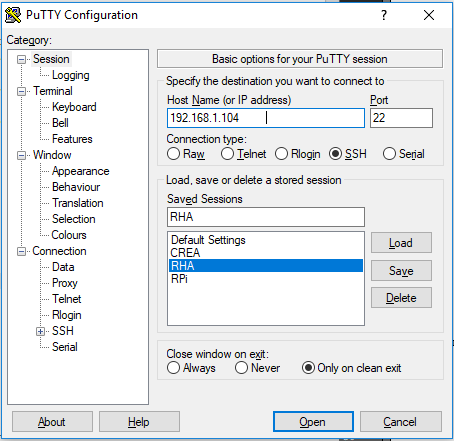
\includegraphics[width=0.5\textwidth]{figuras/Putty.png}
\caption{Interfaz de Putty}
\label{fig:putty}
\end{figure}

\item \textbf{Conexión SSH desde Linux}

En Linux se puede establecer una conexión SSH haciendo uso del terminal

\begin{lstlisting}[frame=single, label=command:ssh]
$ ssh root@190.168.1.104
\end{lstlisting}

El comando \textit{ssh} establece este tipo de conexiones. El usuario se indica en el lugar de \textit{root} en el ejemplo mientras que la IP del remoto se sitúa después del arroba. Es posible configurar el puerto con la opción \textit{-p} (por defecto se usa el puerto 22).

\begin{lstlisting}[frame=single, label=command:ssh-p]
$ ssh -p 22 root@190.168.1.104
\end{lstlisting}

De igual manera que en Windows, se solicitará la contraseña del usuario si procede y se accederá al terminal.

\end{itemize}

\subsection{MQTT}

Mosquitto (Message Queue Telemetry Transport) es un protocolo de código abierto enfocado a las conexiones Machine-to-Machine (M2M) \cite{Vega:2016} que se ha popularizado entre diferentes aplicaciones que precisan de comunicación entre sensores y mandos de redes domóticas. Entre sus características se encuentra un consumo de recursos muy bajo.

Su funcionamiento se basa en una configuración de estrella. Trabaja con un nodo central (también llamado Broker) con el que se establecen conexiones bidireccionales desde múltiples clientes (figura \ref{fig:mqtt}). Estas conexiones son cifradas, aportando una capa de seguridad a la red domótica.

\begin{figure}[tb]
\centering
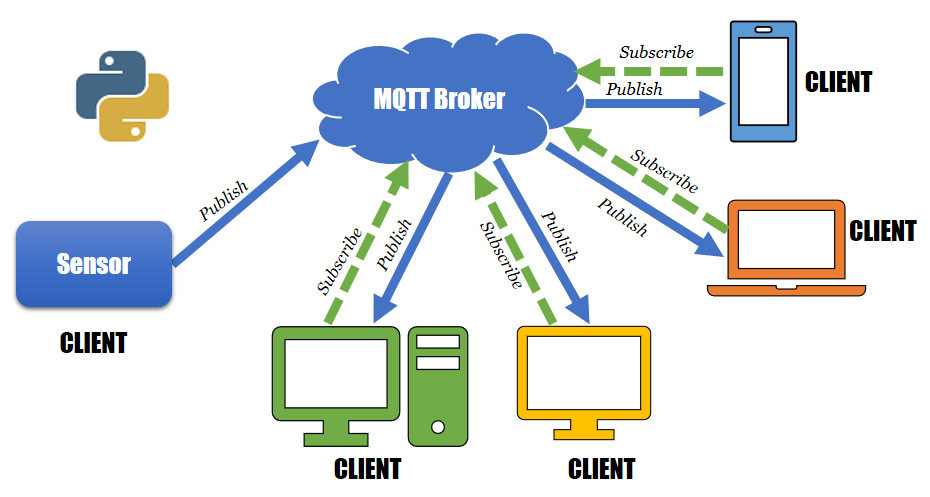
\includegraphics[width=0.75\textwidth]{figuras/mqtt.png}
\caption{Arquitectura MQTT}
\label{fig:mqtt}
\end{figure}

El concepto de \textit{topic} es la forma que tiene MQTT de articular las comunicaciones. Se puede hacer una analogía de los \textit{topic} con un tablón de anuncios. La gente puede publicar en el tablón lo que le plazca y esto será visto por aquellos que se paren a mirar el tablón. De igual manera funciona MQTT, cualquier cliente puede publicar en un \textit{topic} y este mensaje será recibido por aquellos clientes que estén suscritos a ese mismo \textit{topic}. Los \textit{topics}, además, son jerarquizables. Esto es, pueden generarse subtopics de manera recurrente con el fin de poder enviar mensajes únicamente a un grupo de clientes si se observa la red desde una perspectiva más global.

Existen varios \textit{Broker} de MQTT pero, con diferencia, el más popular es el llamado Mosquitto.

Una guía para su instalación puede encontrarse en el Anexo \ref{anexo:mqtt}

\subsubsection{MQTT en RoboHealth}

En cuanto al funcionamiento dentro de la habitación, existe un topic denominado \textit{Robohealth/room/devices} donde publican los distintos dispositivos mientras Node-RED está suscrito.

Los mensajes en el topic de la habitación siguen un mismo formato:

$$\{'id':xx,'atrib1':'yy','atrib2':'zz',(...)\}$$

\textit{xx} remplaza el identificador del cliente, único para cada dispositivo. RoboHealth Arm ha sido identificado con el número \textbf{99}.

\textit{atrib1}, \textit{atrib2} y sucesivos son atributos a los que se les quiere dar un valor. En el caso de los dispositivos digitales el atributo suele ser único, siendo denominado \textit{status}. En el caso de RoboHealth Arm es posible trasladarle dos atributos correspondientes a las coordenadas articulares objetivo del robot. Los atributos son \textbf{shoulder} para el hombro y \textbf{elbow} para el codo.

\textit{yy}, \textit{zz} y sucesivos son los valores correspondientes a los atributos. En el caso del brazo deberán pasarse las dos \textbf{coordenadas articulares en formato hexadecimal}.

\subsection{Node-RED}

Node-RED es una herramienta de programación basada en una interfaz de programación online representada a través de flujos y nodos (figura \ref{fig:nodeinterfaz}). Viene preinstalada en Raspbian Stretch, lo que puede dar una idea del grado de integración que tiene esta herramienta en la comunidad.

Los flujos representan caminos de transmisión de los objetos de node-RED, denominados por defecto \textit{msg}. Estos objetos \textit{msg} poseen unos atributos, algunos creados por defecto y otros opcionales customizados. Uno de los atributos por defecto es \textit{payload}, que suele ser utilizado como contenedor de la información a trasladar. Esta información puede ser de casi cualquier tipo, desde un booleano hasta otro objeto con sus propios atributos. El otro de los atributos por defecto es \textit{\_msgid}, que es un identificador del mensaje enviado que sirve para monitorizar su estado a lo largo del flujo.

Los nodos son etapas en las que, basándose en diferentes tecnologías, se realiza una acción cuando se produce la entrada del mensaje a través del flujo. Esta acción puede ir desde producir algún tipo de reacción ajena a Node-RED hasta modificar variables internas del programa, modificando (o no) el mensaje de flujo antes de volver a transmitirlo.

Existen nodos relacionados con un gran número de tareas. La comunidad puede aportar sus propios paquetes de nodos, ampliando progresivamente el número de tecnologías compatibles con Node-RED. Algunos de los nodos más representativos y usados en el proyecto Robohealth son los siguientes:

\begin{figure}[H]
\centering
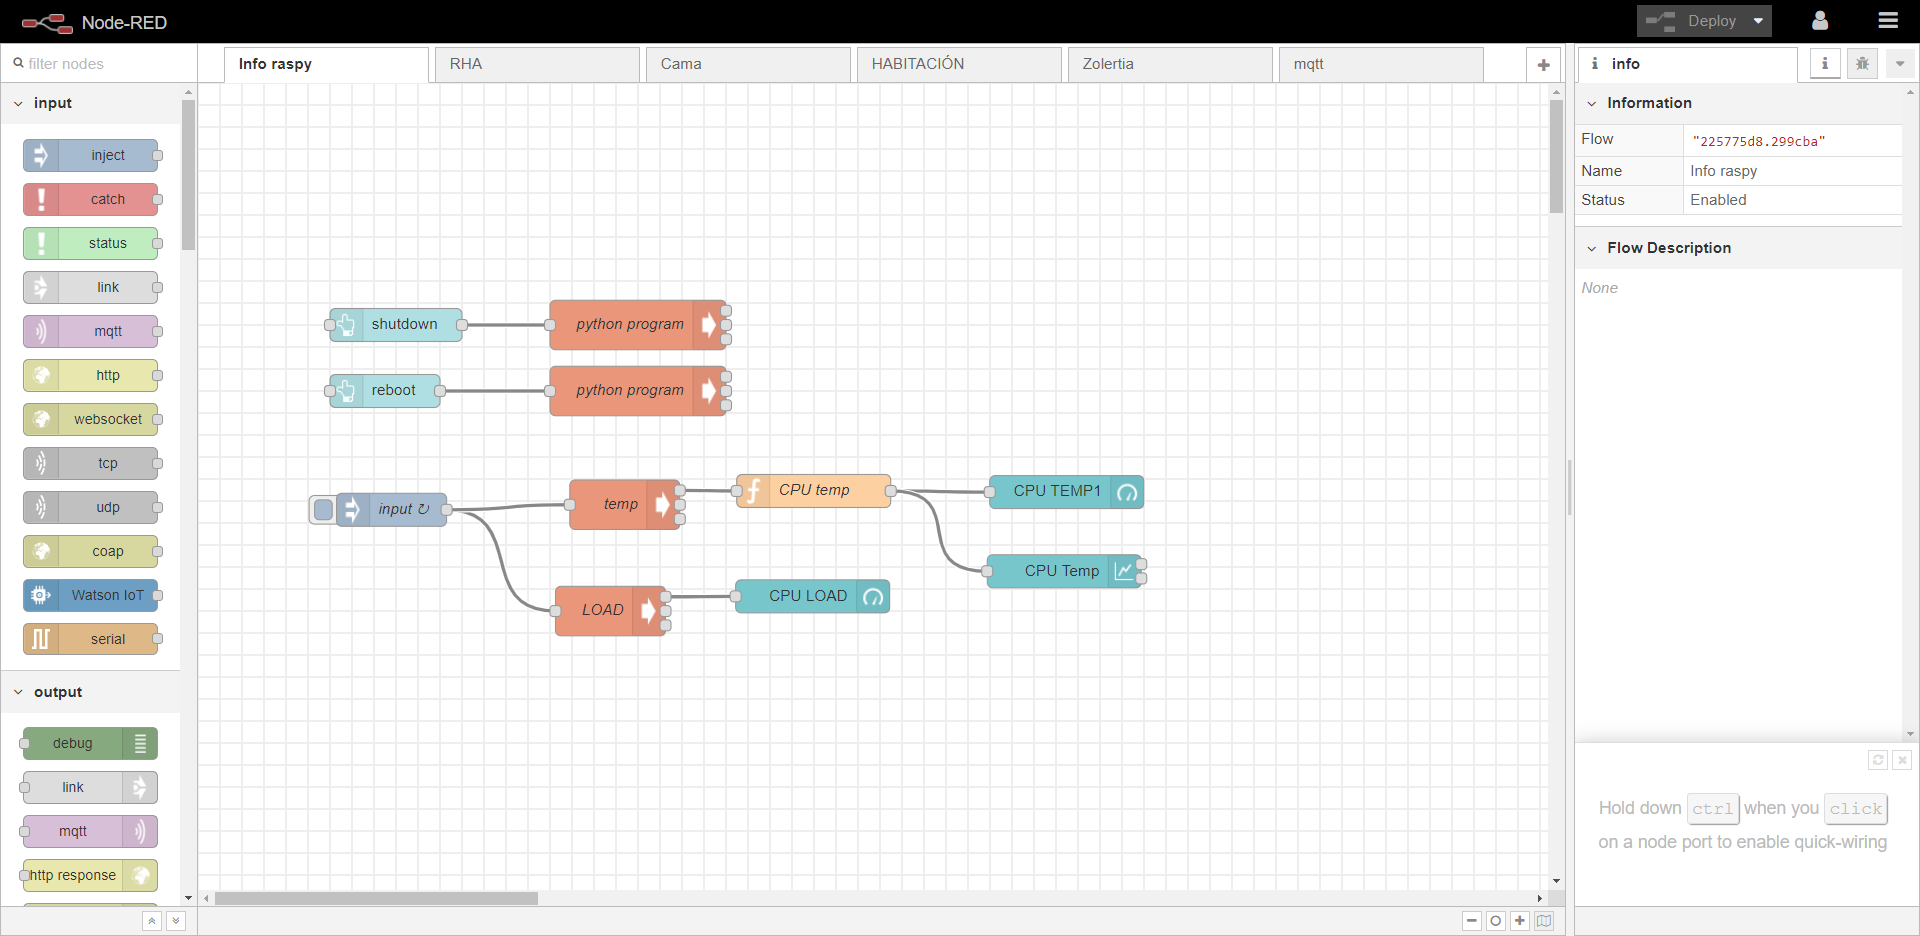
\includegraphics[width=0.7\textwidth]{figuras/InterfazNodeRed.png}
\caption{Ejemplo de interfaz de Node-RED}
\label{fig:nodeinterfaz}
\end{figure}

\begin{itemize}
\item \textbf{Debug node}

El nodo \textit{Debug} (figura \ref{fig:nodedebug}) representa una imagen del objeto \textit{msg} o de uno de sus atributos a su paso por un punto concreto del flujo. Normalmente hace uso de la pestaña debug de la interfaz de Node-RED.

\begin{figure}[H]
  \centering
  \begin{minipage}[b]{0.3\textwidth}
    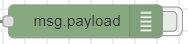
\includegraphics[width=\textwidth]{figuras/debugNode.png}
    \subcaption{Representación}
  \end{minipage}
  \hfill
  \begin{minipage}[b]{0.5\textwidth}
    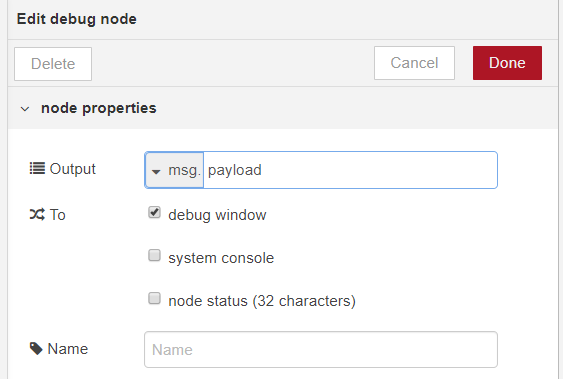
\includegraphics[width=\textwidth]{figuras/debugNodeProp.png}
    \subcaption{Configuración}
  \end{minipage}
  \caption{Nodo Debug}\label{fig:nodedebug}
\end{figure}

\item \textbf{Function node}

El nodo \textit{Function} (figura \ref{fig:nodefunction}) contiene una función programada en JavaScript que, por convenio, recibe el objeto \textit{msg} proveniente del flujo y lo utiliza para crear un nuevo objeto (u objetos) \textit{message} que pasar al siguiente nodo del flujo. Existe la posibilidad de no devolver nada si se desea congelar el flujo en ciertas situaciones.

\begin{figure}[H]
\centering
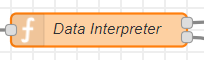
\includegraphics[width=0.5\textwidth]{figuras/fcnNode.png}
\caption{Nodo Function}
\label{fig:nodefunction}
\end{figure}

\item \textbf{Exec node}

El nodo \textit{Exec} (figura \ref{fig:nodeexec}) es el nodo de ejecución de comandos. El comando a ejecutar se define en las propiedades, siendo posible añadir el mensaje recibido a través del flujo al final del comando. Las salidas del bloque corresponden a \textit{stdout}, \textit{stderr} y a objetos devueltos. Es posible configurar si la salida debe volcarse al final de la ejecución o en directo durante la ejecución del programa.

\begin{figure}[H]
  \centering
  \begin{minipage}[b]{0.3\textwidth}
    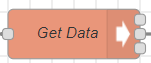
\includegraphics[width=\textwidth]{figuras/execNode.png}
    \subcaption{Representación}
  \end{minipage}
  \hfill
  \begin{minipage}[b]{0.5\textwidth}
    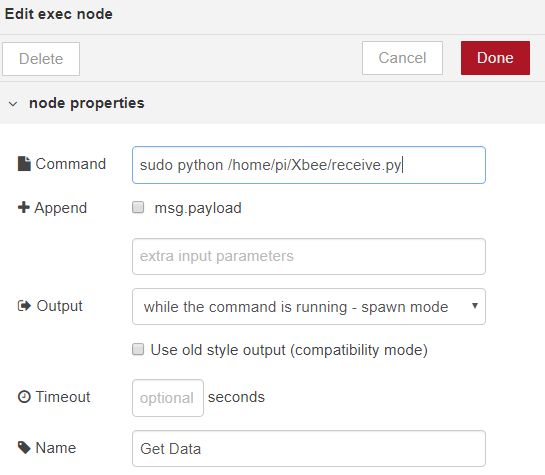
\includegraphics[width=\textwidth]{figuras/execNodeProp.png}
    \subcaption{Configuración}
  \end{minipage}
  \caption{Nodo Debug}\label{fig:nodeexec}
\end{figure}

\item \textbf{MQTT node}

Algunos de los nodos desarrollados por terceros son los relacionados con MQTT. Existen nodos de entrada de MQTT (figura \ref{fig:nodeMQTT}) y nodos de salida. La configuración disponible incluye la IP, el puerto y el \textit{topic} al que suscribirse o publicar.

\begin{figure}[H]
  \centering
  \begin{minipage}[b]{0.3\textwidth}
    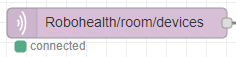
\includegraphics[width=\textwidth]{figuras/MQTTNode.png}
    \subcaption{Representación}
  \end{minipage}
  \hfill
  \begin{minipage}[b]{0.5\textwidth}
    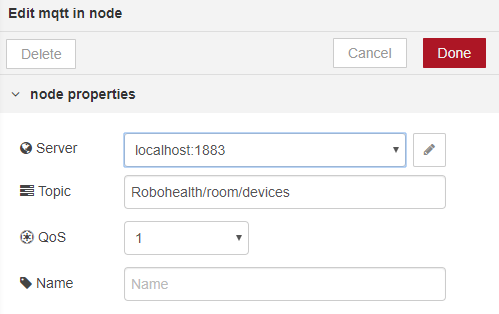
\includegraphics[width=\textwidth]{figuras/MQTTNodeProp.png}
    \subcaption{Configuración}
  \end{minipage}
  \caption{Nodo entrada MQTT}\label{fig:nodeMQTT}
\end{figure}

\item \textbf{Nodos de gestión de flujo}

Una serie de nodos se usan para modificar el comportamiento normal del flujo de los mensajes \textit{msg}. Posibilitan la aplicación de cierta lógica al programa.

\begin{itemize}

\item \textbf{Inject node}

El nodo de inyección introduce un mensaje en el flujo. Se puede programar una inyección periódica, que haga funcionar el flujo de manera similar a un bucle software.

\begin{figure}[H]
  \centering
  \begin{minipage}[b]{0.3\textwidth}
    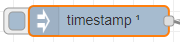
\includegraphics[width=\textwidth]{figuras/injectNode.png}
    \subcaption{Representación}
  \end{minipage}
  \hfill
  \begin{minipage}[b]{0.5\textwidth}
    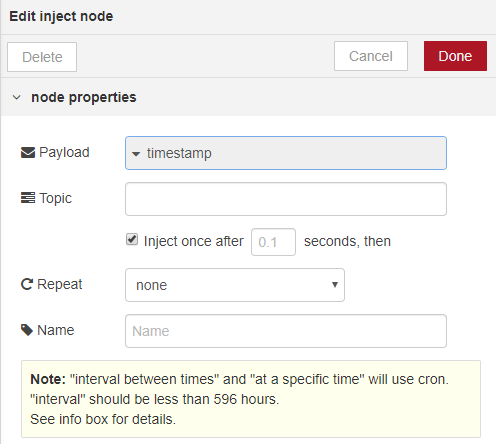
\includegraphics[width=\textwidth]{figuras/injectNodeProp.png}
    \subcaption{Configuración}
  \end{minipage}
  \caption{Nodo Inject}\label{fig:nodeinject}
\end{figure}

\item \textbf{Delay node}

El nodo \textit{Delay} detiene la ejecución del programa durante el tiempo especificado.

\begin{figure}[H]
  \centering
  \begin{minipage}[b]{0.3\textwidth}
    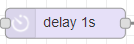
\includegraphics[width=\textwidth]{figuras/delayNode.png}
    \subcaption{Representación}
  \end{minipage}
  \hfill
  \begin{minipage}[b]{0.5\textwidth}
    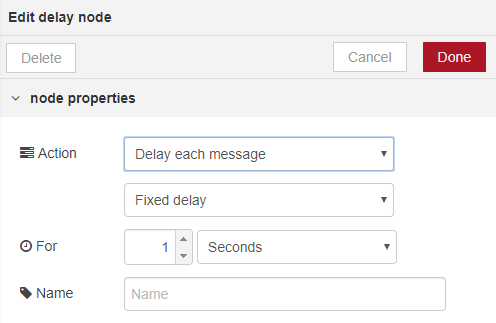
\includegraphics[width=\textwidth]{figuras/delayNodeProp.png}
    \subcaption{Configuración}
  \end{minipage}
  \caption{Nodo Delay}\label{fig:nodedelay}
\end{figure}

\item \textbf{Switch node}

El nodo \textit{Switch} compara algún atributo del mensaje \textit{msg} con unos valores programados y asignados a cada una de las salidas. Es equivalente a la expresión condicional \textit{switch-case}.

\begin{figure}[H]
  \centering
  \begin{minipage}[b]{0.3\textwidth}
    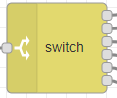
\includegraphics[width=\textwidth]{figuras/switchNode.png}
    \subcaption{Representación}
  \end{minipage}
  \hfill
  \begin{minipage}[b]{0.5\textwidth}
    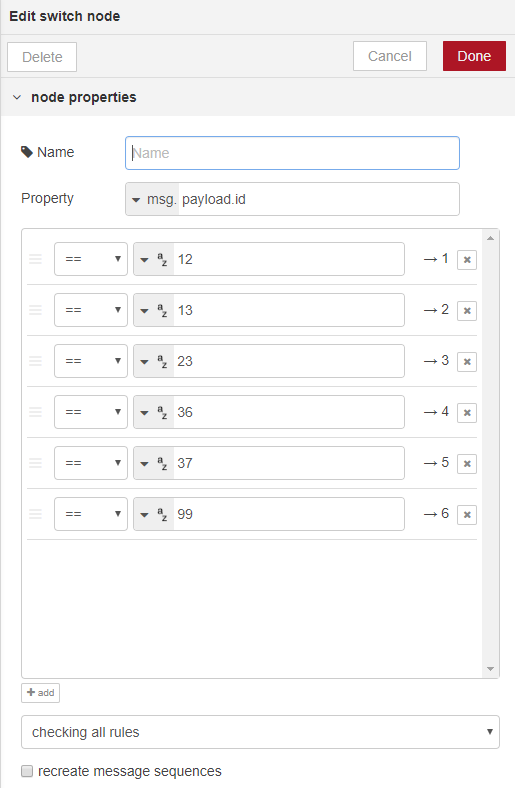
\includegraphics[width=\textwidth]{figuras/switchNodeProp.png}
    \subcaption{Configuración}
  \end{minipage}
  \caption{Nodo Switch}\label{fig:nodeexec}
\end{figure}

\end{itemize}


\item \textbf{Nodos de UI}

Existen varios nodos que representan objetos en el Dashboard de Node-RED que sirve de interfaz gráfica. Estos nodos pueden ser de entrada o salida de información

\begin{itemize}
\item \textbf{Ejemplos de nodos de entrada}

Los nodos de entrada (figura \ref{fig:nodeinput}) permiten introducir mensajes en el sistema. Existen entradas digitales, como pueden ser botones o interruptores, o entradas analógicas, como sliders.

\begin{figure}[H]
  \centering
  \begin{minipage}[t]{0.3\textwidth}
    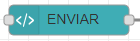
\includegraphics[width=\textwidth]{figuras/templateNode.png}
    \subcaption{Nodo Template}
  \end{minipage}
  \hfill
  \begin{minipage}[t]{0.4\textwidth}
    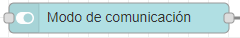
\includegraphics[width=\textwidth]{figuras/switchinputNode.png}
    \subcaption{Nodo interruptor}
  \end{minipage}
  \begin{minipage}[b]{0.3\textwidth}
    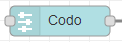
\includegraphics[width=\textwidth]{figuras/sliderNode.png}
    \subcaption{Nodo Slider}
  \end{minipage}
  \hfill
  \begin{minipage}[b]{0.3\textwidth}
    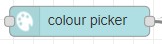
\includegraphics[width=\textwidth]{figuras/colourNode.png}
    \subcaption{Nodo selector de color}
  \end{minipage}
  \caption{Nodos de entrada}\label{fig:nodeinput}
\end{figure}

\item \textbf{Ejemplos de nodos de salida}

Los nodos de salida (figura \ref{fig:nodeoutput}) representan el valor de algún atributo del mensaje que les llega. Esta representación puede tener formato de texto, numérico o gráfico.

\begin{figure}[H]
  \centering
  \begin{minipage}[t]{0.3\textwidth}
    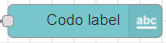
\includegraphics[width=\textwidth]{figuras/textNode.png}
    \subcaption{Nodo de texto}
  \end{minipage}
  \hfill
  \begin{minipage}[t]{0.3\textwidth}
    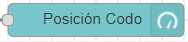
\includegraphics[width=\textwidth]{figuras/gaugeNode.png}
    \subcaption{Nodo gráfico}
  \end{minipage}
  \hfill
  \begin{minipage}[t]{0.3\textwidth}
    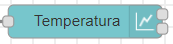
\includegraphics[width=\textwidth]{figuras/chartNode.png}
    \subcaption{Nodo Chart}
  \end{minipage}
  %\hfill
  \caption{Nodos de salida}\label{fig:nodeoutput}
\end{figure}

\end{itemize}
\end{itemize}

\subsubsection{Node-RED en RoboHealth}

La aplicación de Node-RED para los dispositivos de RoboHealth se orienta a la interacción con el usuario a través de una interfaz gráfica. Esta interfaz gráfica se divide en dos layout.

El primer layout (figura \ref{fig:infoRaspyDash}) se encarga del control básico del estado de la Raspberry Pi. Incluye representaciones de la temperatura y el uso de la CPU así como botones para reiniciar y apagar el ordenador.

\begin{figure}[H]
\centering
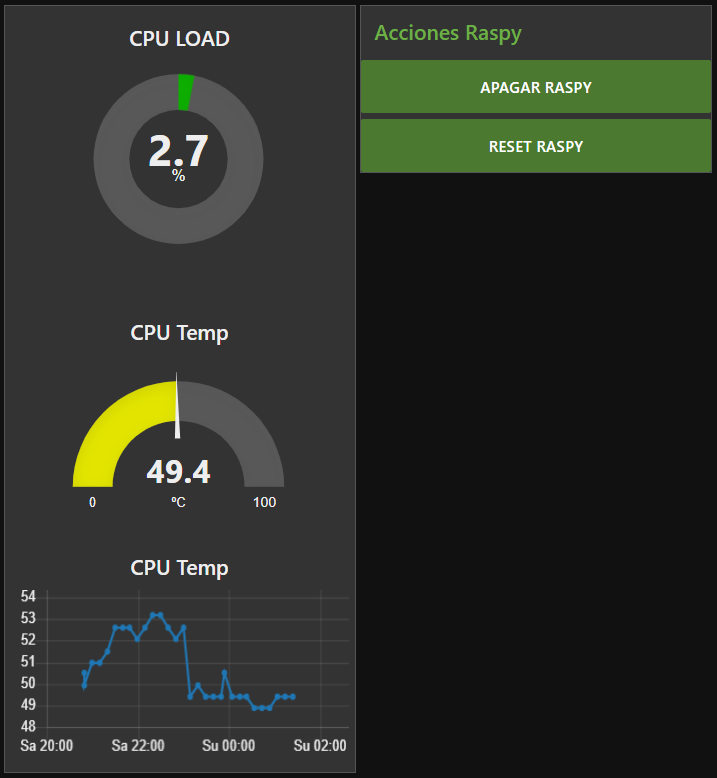
\includegraphics[width=0.7\textwidth]{figuras/infoRaspyDash.png}
\caption{UI de control elemental}
\label{fig:infoRaspyDash}
\end{figure}

El flujo (figura \ref{fig:infoRaspyFlow}) se basa en la ejecución de comandos para obtener la información de temperatura (línea 1/código \ref{comando:infoRaspy}) y carga de la CPU (línea 2/código \ref{comando:infoRaspy}). De igual manera, se lanzan comandos para apagar (línea 3/código \ref{comando:infoRaspy}) y reiniciar (línea 4/código \ref{comando:infoRaspy}) la Raspberry Pi. Los comandos utilizados son los siguientes:

% Configuración de la visualización del código SW
\lstset{backgroundcolor=\color{verde_p},numbers=left,numberstyle=\tiny, language=bash, breaklines=true, basicstyle=\footnotesize, xleftmargin=25pt, framesep=8pt, numbersep=15pt}

\begin{lstlisting}[frame=single, label=command:ssh, label=comando:infoRaspy]
$ vcgencmd measure_temp
$ top -d 0.5 -b -n2 | grep "Cpu(s)"|tail -n 1 | awk '{print $2 + $4}'
$ sudo shutdown -h now
$ sudo reboot
\end{lstlisting}

\begin{figure}[tb]
\centering
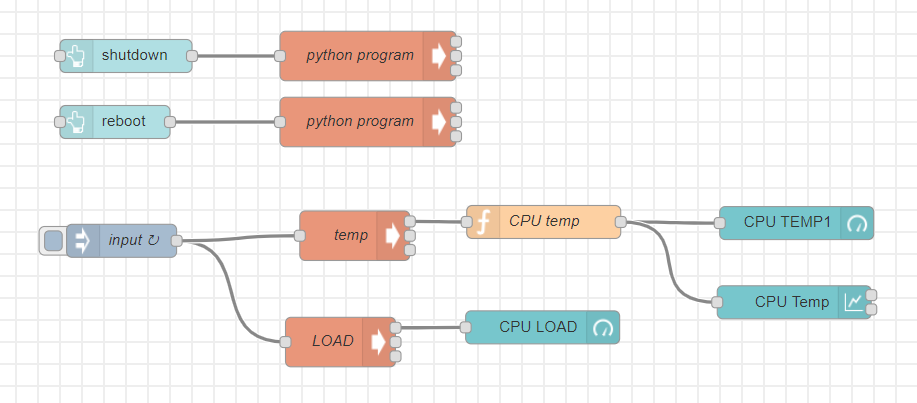
\includegraphics[width=0.9\textwidth]{figuras/infoRaspyFlow.png}
\caption{Flujo de control elemental}
\label{fig:infoRaspyFlow}
\end{figure}

El segundo layout incluye el control de los dispositivos previamente desarrollado. El Dashboard (figura \ref{fig:Dashboard}) recoge la UI para controlar cada bloque de dispositivos. A continuación se recogen ejemplos de los flujos correspondientes a la cama (figura \ref{fig:camaFlow}), la habitación (figura \ref{fig:persianasFlow}\footnote{En la imagen se recoge únicamente el flujo correspondiente a las persianas}) o los dispositivos Zolertia (figura \ref{fig:zolertiaFlow}).

\begin{figure}[tb]
\centering
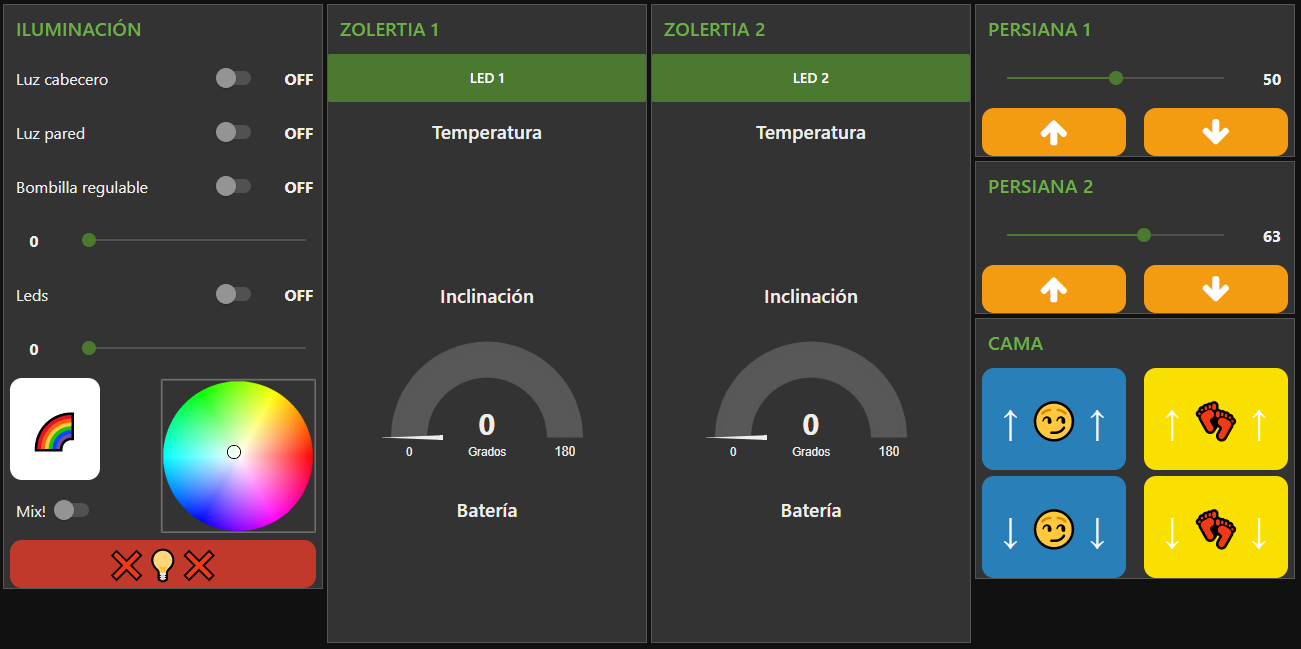
\includegraphics[width=0.8\textwidth]{figuras/Dashboard.png}
\caption{Dashboard}
\label{fig:Dashboard}
\end{figure}

\begin{figure}[H]
\centering
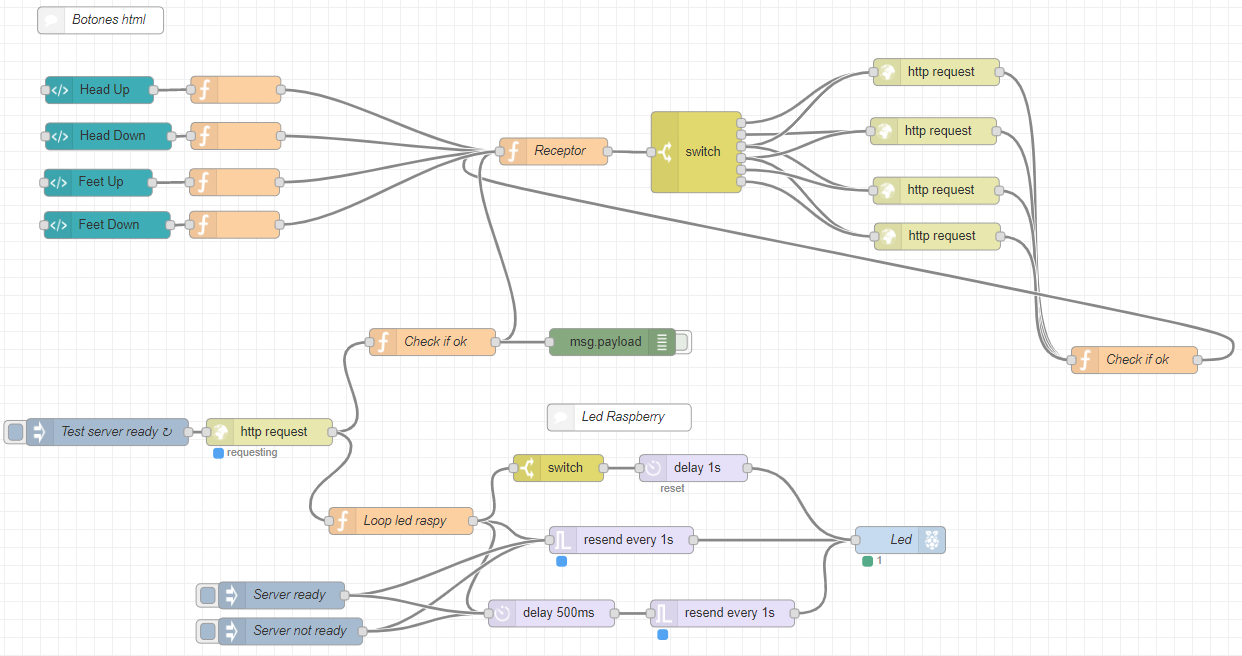
\includegraphics[width=1\textwidth]{figuras/camaFlow.png}
\caption{Flujo de control de la cama}
\label{fig:camaFlow}
\end{figure}

\begin{figure}[H]
\centering
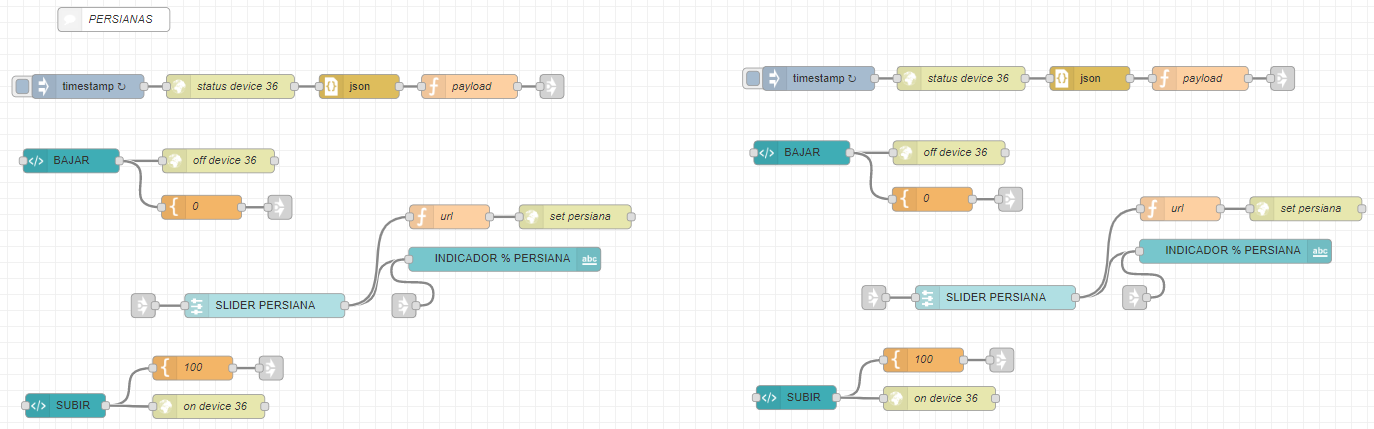
\includegraphics[width=1\textwidth]{figuras/persianasFlow.png}
\caption{Flujo de control de las persianas}
\label{fig:persianasFlow}
\end{figure}

\begin{figure}[H]
\centering
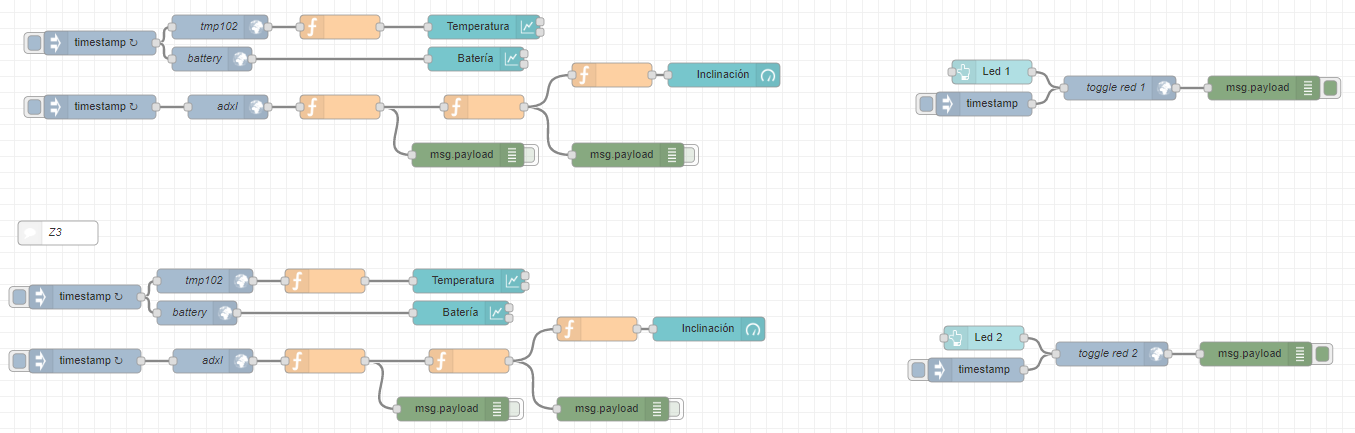
\includegraphics[width=1\textwidth]{figuras/zolertiaFlow.png}
\caption{Flujo de control de Zolertia}
\label{fig:zolertiaFlow}
\end{figure}

\subsubsection{Node-RED para RoboHealth Arm}

Para el control de RoboHealth Arm se ha desarrollado un flujo en Node-RED que se explica a continuación.

En la figura \ref{fig:ONOFFRHA} se muestra el flujo de encendido del brazo robótico

\begin{figure}[H]
\centering
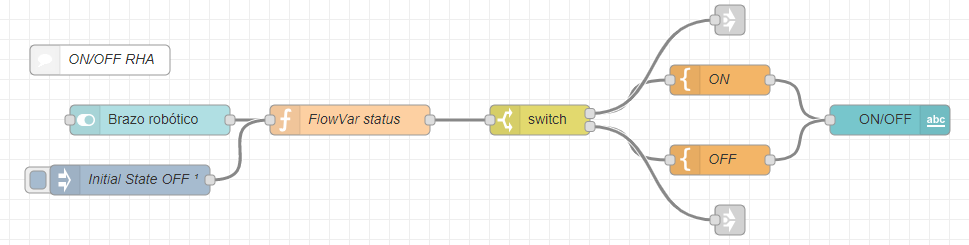
\includegraphics[width=0.9\textwidth]{figuras/ONOFFFlowRHA.png}
\caption{Flujo de encendido de RHA}
\label{fig:ONOFFRHA}
\end{figure}

El flujo se basa en la obtención el estado del control del brazo a través del botón ON/OFF y su asignación a una variable de flujo. Esta asignación se efectúa a través de la función \textit{FlowVar status} (código \ref{code:FlowVarStatus})

% Esto para configurar como se va a visualizar el código
\lstset{backgroundcolor=\color{amarillo_claro}, numbers=left,numberstyle=\tiny, language=Java, breaklines=true, basicstyle=\footnotesize, xleftmargin=25pt, framesep=8pt, numbersep=15pt}


\begin{lstlisting}[frame=leftline, caption={FlowVar status}, label=code:FlowVarStatus]
if (msg.payload === true) {
    flow.set("status","ON");
}
else if (msg.payload === false) {
    flow.set("status","OFF");
}
msg.payload = flow.get("status");
return msg;
\end{lstlisting}

Se incluye también en el flujo la inyección del estado inicial OFF al comenzar la ejecución.

El flujo de recepción de la información de RHA se programa como en la figura \ref{fig:RecepcionRHA}

\begin{figure}[H]
\centering
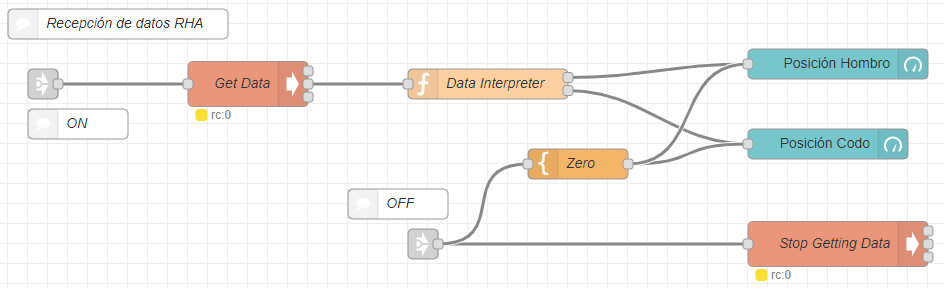
\includegraphics[width=0.9\textwidth]{figuras/RecepcionFlowRHA.png}
\caption{Flujo de recepción de RHA}
\label{fig:RecepcionRHA}
\end{figure}

La recepción de un flanco de encendido, pone a correr el comando \ref{comand:getDataRHA} que lanza un script que devuelve los datos recibidos. Estos datos se interpretan con la función \textit{Data interpreter} (código \ref{code:DataInterpreter}) y se muestra la información en el Dashboard con una salida gráfica

% Configuración de la visualización del código SW
\lstset{backgroundcolor=\color{verde_p}, numbers=none, language=bash, breaklines=true, basicstyle=\footnotesize, xleftmargin=25pt, framesep=8pt, numbersep=15pt}

\begin{lstlisting}[frame=single, label=command:getDataRHA]
$ sudo python /home/pi/Xbee/receive.py
\end{lstlisting}

% Esto para configurar como se va a visualizar el código
\lstset{backgroundcolor=\color{amarillo_claro}, numbers=left,numberstyle=\tiny, language=Java, breaklines=true, basicstyle=\footnotesize, xleftmargin=25pt, framesep=8pt, numbersep=15pt}

\begin{lstlisting}[frame=leftline, caption={Data Interpreter}, label=code:DataInterpreter]
var num1_str = msg.payload[1]+msg.payload[2]+msg.payload[3];
if (msg.payload.length < 11) {
    var num2_str = msg.payload[6]+msg.payload[7];
}
else {
    var num2_str = msg.payload[6]+msg.payload[7]+msg.payload[8];
}
msg.payload = num1_str;
var newMsg = {payload: num2_str}
return [msg, newMsg];
\end{lstlisting}

Un flanco de apagado detiene el script con el comando \ref{comand:stopGettingDataRHA} y manda un 0 a la representación de la información

% Configuración de la visualización del código SW
\lstset{backgroundcolor=\color{verde_p}, numbers=none, language=bash, breaklines=true, basicstyle=\footnotesize, xleftmargin=25pt, framesep=8pt, numbersep=15pt}

\begin{lstlisting}[frame=single, label=command:stopGettingDataRHA]
$ sudo pkill -f receive.py
\end{lstlisting}

El flujo de configuración de la emisión de datos se encuentra en la figura \ref{fig:configRHA}. En resumen, obtiene los datos de posiciones articulares y modo de comunicación de la interfaz gráfica y los asigna a variables de flujo. Las posiciones articulares están limitadas por los slider: para el codo, los valores estan entre \textbf{60 y 110}; para el hombro, entre \textbf{125 y 166}. Las funciones \textit{FlowVar elbow}, \textit{FlowVar shoulder} y \textit{FlowVar ComMode} son similares a \textit{FlowVar status} (código \ref{code:FlowVarStatus}). El flujo también establece los valores iniciales para codo, hombro y modo de comunicación; siendo 60, 125 y AT respectivamente.

\begin{figure}[H]
\centering
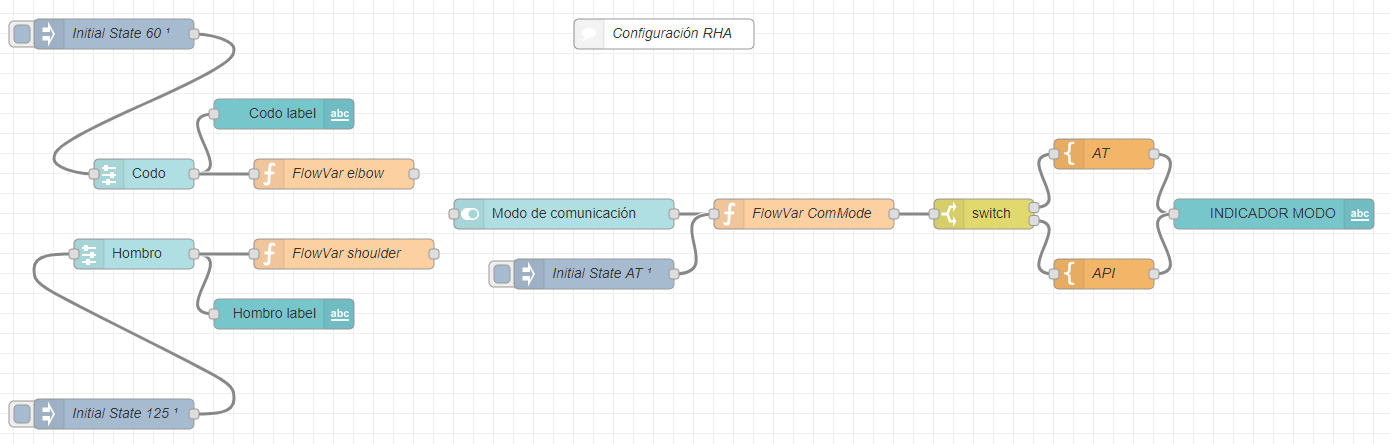
\includegraphics[width=0.9\textwidth]{figuras/configFlowRHA.png}
\caption{Flujo de configuración de RHA}
\label{fig:configRHA}
\end{figure}

En la figura \ref{fig:emisionRHA} se recoge el flujo correspondiente a la emisión de datos al RHA. Comprueba el tipo de comunicación y elige el script a correr de acuerdo a ello. Previamente, obtiene las coordenadas articulares para pasárselas a los scripts.

\begin{figure}[H]
\centering
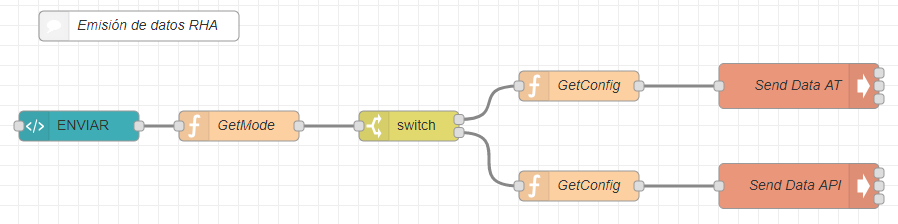
\includegraphics[width=0.9\textwidth]{figuras/emisionFlowRHA.png}
\caption{Flujo de emisión de RHA}
\label{fig:emisionRHA}
\end{figure}

Función \textit{GetMode}:

% Esto para configurar como se va a visualizar el código
\lstset{backgroundcolor=\color{amarillo_claro}, numbers=left,numberstyle=\tiny, language=Java, breaklines=true, basicstyle=\footnotesize, xleftmargin=25pt, framesep=8pt, numbersep=15pt}

\begin{lstlisting}[frame=leftline, caption={GetMode}, label=code:GetMode]
if (flow.get("ComMode") === undefined) {
    flow.set("ComMode","AT");
}
if (flow.get("status") == "ON") {
    msg.payload = flow.get("ComMode");
}
return msg;
\end{lstlisting}

Función \textit{GetConfig}:

\begin{lstlisting}[frame=leftline, caption={GetConfig}, label=code:GetConfig]
var posX = flow.get("RHA_shoulder");
var posY = flow.get("RHA_elbow");
var hex_posX = posX.toString(16);
var hex_posY = posY.toString(16);
msg.payload = [hex_posX,hex_posY];
return msg;
\end{lstlisting}

Comandos para enviar los mensajes AT y API. En la práctica, \textit{msg.payload} se añade al final del comando.

% Configuración de la visualización del código SW
\lstset{backgroundcolor=\color{verde_p}, numbers=none, language=bash, breaklines=true, basicstyle=\footnotesize, xleftmargin=25pt, framesep=8pt, numbersep=15pt}

\begin{lstlisting}[frame=single, label=command:sendDataRHA]
$ sudo python /home/pi/Xbee/send-AT.py
$ sudo python /home/pi/Xbee/send-API.py
\end{lstlisting}

\subsection{Python scripts}

En la Raspberry Pi están guardados una serie se scripts en lenguaje Python que son los encargados de enviar (tanto en modo AT, como en modo API) y recibir la información.

Unos comentarios sobre la edición y compilación de scripts escritos en Python en una máquina que corra Raspbian y, en general, cualquier sistema operativo basado en GNU/Linux, pueden ser encontrados en el Anexo \ref{anexo:scripts}.

A continuación se explica detalladamente cada uno de estos scripts.

\subsubsection{SendAT.py}\label{subsubsec:sendat}

Es un script encargado de enviar comandos en modo AT hacia el puerto serial adecuado. El \textbf{código íntegro de SendAT.py} se puede encontrar en el Anexo \ref{anexo:sendAT}.

En las primeras 5 líneas se importan las librerías necesarias. Se puede observar que hacemos uso de la librería del sistema, para acceder a los atributos pasados con el comando; a la librería de tiempo, relacionada con el los timestamps del logging de la información realizado a través de la librería \textit{logging}; y a la librería \textit{serial} para poder acceder a esos puertos.

En la línea 7 se configura el log de la información. Se establece el archivo \textit{/home/pi/Xbee/SendLogs/sentAT.log} como archivo de destino, se desactivan restricciones de nivel\footnote{Las restricciones de nivel son barreras a la introducción de ciertos tipos de mensajes en el archivo de destino en función de su importancia (ERROR/WARNING/INFO)} y, por último, se determina el formato del mensaje que incluye un timestamp al inicio.

Entre las líneas 9 y 16 se abre una comunicación serial con el puerto \textit{/dev/ttyACM0}\footnote{Linux detecta como un dispositivo en un puerto \textit{ttyACM*} a aquellos dispositivos de comunicación USB del subtipo \textit{"Abstract Control Mode"}. Arduino se encuentra en esta categoría} a una tasa de baudios de 115200. El resto de la configuración entra dentro de los parámetros usuales y por defecto.

De la línea 18 a 22 se comprueba que el número de argumentos pasados es el adecuado. De lo contrario, se simulan unos argumentos neutrales genéricos y se guarda un \textit{Warning} en el archivo de log. Si los argumentos se han pasado de manera correcta, se sacan del atributo del sistema.

En las líneas 24-27 se obtienen los números enteros a partir de los argumentos hexadecimales de entrada.

En la línea 28 se calcula el checksum de acuerdo al protocolo de comunicación de RHA.

A partir de la línea 30, se comprueba que los valores introducidos están dentro del rango admisible para el brazo robótico, se integra un frame y se escribe por serial; guardando el resultado de la operación en el archivo de log.

Las características del modo AT se explican en el apartado \ref{subsubsec:modoscom}.

\subsubsection{SendAPI.py}\label{subsubsec:sendapi}

Se trata de un script que, de igual manera que SendAT.py, envía datos hacia un puerto serial, pero esta vez encuadrado dentro del modo API. Este modo modifica la estructura del frame enviado. El \textbf{código íntegro de SendAPI.py} puede ser encontrado en el Anexo \ref{anexo:sendAPI}.

El código es similar al de SendAT.py. De hecho, hasta la línea 29, es exactamente igual a excepción de configurar el archivo \textit{/home/pi/Xbee/SendLogs/sentAPI.log} como archivo de destino del log de información.

En la línea 30, se encuentra el cálculo del checksum de necesario para el modo API.

Entre las líneas 32 y 41 se forma el frame de acuerdo a las necesidades API y se envía por serial; guardando el resultado en el log.

Las características del modo API y sus diferencias con el modo AT se explican en el apartado \ref{subsubsec:modoscom}.

\subsubsection{Receive.py}\label{subsubsec:receive}

Receive.py es el script encargado de obtener los frames recibidos por serial. El \textbf{código íntegro de receive.py} puede ser encontrado en el Anexo \ref{anexo:receive}.

Se configura el log de información con salida hacia el archivo \textit{/home/pi/Xbee/ReceiveLogs/receiveAT.log}. La configuración del puerto serial es igual a la indicada en los dos scripts anteriores.

Entre las líneas 19 y 25, se puede encontrar la función \textit{serialReader()} que se encarga de leer un byte por serial y transformarlo a entero. Para este proceso, es necesario importar la librería \textit{struct}, cuyo método \textit{unpack()} sirve de mucha utilidad. Devuelve -1 si no se lee nada por serial.

A partir de la línea 27, se puede observar un bucle infinito que comprueba las lecturas por serial hasta dar con un frame del brazo. Una vez encontrado este frame, lo guarda en el archivo de log y extrae las posiciones articulares. Imprime estas dos posiciones como vector por la salida de error \textit{stderr} por necesidades externas explicadas en el apartado \ref{subsec:NR-Xbee}.

\section{Transmisión de la información}

Para la transmisión de la información, se eligió utilizar tecnología basada en la radiofrecuencia con el objetivo de diversificar la naturaleza de los dispositivos presentes en la habitación del proyecto RoboHealth.

Dentro de la radiofrecuencia, existen varios tipos de dispositivos y plataformas que pueden ayudarnos en nuestro objetivo. Un resumen de estas alternativas con sus características puede ser encontrado en la tabla \ref{tab:radio}.

\begin{table}[H]
\begin{center}
\begin{tabular}{|m{3cm}|m{1cm}|m{7cm}|}
\hline
\textbf{Nombre} & \multicolumn{2}{|c|}{\textbf{Características}}\\
\hline
\hline
\multirow{2}{3cm}{XBee} & Pros & Mucha documentación, variedad de versiones, precio contenido, versatilidad\\
\cline{2-3}
& Cons & Sobredimensionado\\
\hline
\multirow{2}{3cm}{Jennic JN5148} & Pros & Menor tamaño, coste contenidos\\
\cline{2-3}
& Cons & Dificil distribución, documentación limitada\\
\hline
\multirow{2}{3cm}{HPZB01W} & Pros & Precio contenido\\
\cline{2-3}
& Cons & Comunicación lenta, difícil manejo y escasa documentación\\
\hline
\multirow{2}{3cm}{RFM12B} & Pros & Coste muy reducido\\
\cline{2-3}
& Cons & Escasa potencia, muy pequeña versatilidad\\
\hline
\end{tabular}
\end{center}
\caption{Alternativas de radiofrecuencia}
\label{tab:radio}
\end{table}

Finalmente, se decidió optar por los módulos XBee. Además de que sus características los hacen perfectamente funcionales para el desarrollo del presente proyecto y las alternativas no eran especialmente buenas, el departamento ya contaba con un par de estos módulos.

\subsection{Módulos XBee}

Los módulos XBee \cite{Xbee:2019} (figura \ref{fig:Xbee}) son un conjunto de pequeños productos orientados a solucionar redes inalámbricas para la comunicación entre dispositivos. Entre sus características se encuentran:

\begin{itemize}
\item Gran variedad de productos que recorren un rango muy amplio tanto de consumos de potencia como de alcances.
\item Son módulos que ofrecen un alto tráfico de datos
\item Baja latencia en la comunicación
\item Precisan una sicronización de comunicación predecible
\item Su aplicación principal es la creación de redes \textit{punto a punto} o \textit{punto a multipunto}.
\end{itemize}

Los módulos XBee trabajan sobre la especificación \textbf{Zigbee} \cite{Zigbee:2019}, que proporciona una alianza y un estandar sobre el que trabajar en redes \textit{mesh} de comunicación. Esta especificación se basa en el estándar IEEE 802.15.4 \cite{IEEE:2007}, que define características físicas como el mecanismo DSSS para la modulación en radiofrecuencia (Se pueden encontrar más detalles en la sección \ref{sec:radiofrec}).

Los módulos XBee de los que se disponen son los denominados XBee S2\cite{XbeeS2:2007}, permiten dos modos de comunicación (apartado \ref{subsubsec:modoscom}) y una infinidad de parámetros configurables (apartado \ref{subsubsec:xctu}). Estos módulos sólo funcionan con módulos de la mismo Serie 2, por lo que todos los dispositivos miembros de la red deben incluir este tipo de módulos.

El módulo XBee S2 trabaja a 3.3V de tensión de alimentación, el layout físico puede consultarse en la figura \ref{fig:XBLayout} y su pinout puede encontrarse en la figura \ref{fig:XBPinout}.

\begin{figure}[tb]
\centering
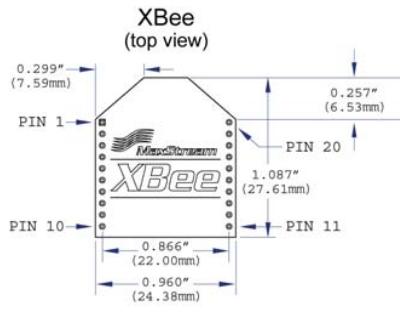
\includegraphics[width=0.5\textwidth]{figuras/XBeeLayout.png}
\caption{Layout del XBee S2}
\label{fig:XBLayout}
\end{figure}

\begin{figure}[bt]
\centering
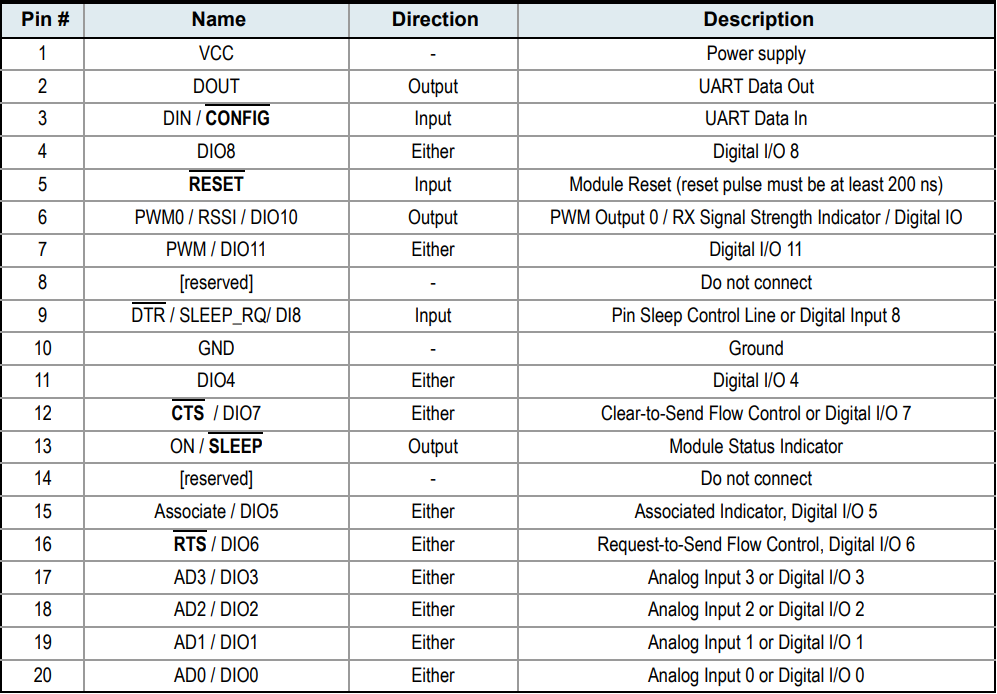
\includegraphics[width=0.9\textwidth]{figuras/XBeePinout.png}
\caption{Pinout del XBee S2}
\label{fig:XBPinout}
\end{figure}

Toda la información relacionada con los módulos de radiofracuencia de Digi puede consultarse en el PDF destinado a ello\cite{Digi:2018} que puede encontrarse en internet.

\subsubsection{Modos de comunicación}\label{subsubsec:modoscom}

Como se ha comentado con anterioridad, existen dos modos de comunicación que pasan a desarrollarse a continuación. Es destacable el hecho de que los modos de comunicación deben coincidir entre los extremos comunicados para que la interpretación o el propio proceso de comunicación sea efectivo.

\begin{itemize}
\item \textbf{Modo AT}

En el modo AT o modo transparente, el módulo actúa como una simple sustitución de la comunicación serial.

Cuando cualquier tipo de información es recibida por radiofrecuencia, es directamente trasladada al pin DOUT del módulo.

Cuando se recibe información a través del pin DIN, se transmite por radiofrecuencia drectamente a las direcciones definidas en la configuración (apartado \ref{subsubsec:xctu}).

Este método es el más simple pero, si en la red existen más de dos módulos XBee y se quiere discriminar la transmisión de información entre uno y otro, los módulos requieren ser reconfigurados a través de los registros de las direcciones de destino. En ese caso, limita mucho la facilidad de la operación.

Se puede comprobar que el script SendAT.py (apartado \ref{subsubsec:sendat}) envía exclusivamente los bytes correspondientes al protocolo de comunicación RHA. La recepción (apartado \ref{subsubsec:receive}) también está pensado para recibir en modo AT, ya que se trata de ser lo menos intrusivo posible en el código fuente del brazo robótico y éste no está preparado para transmitir en modo API.

\item \textbf{Modo API}

El modo API (\textit{Application Programming Interface}) es una alternativa al modo transparente que enmarca la emisión de datos en una serie de mensajes estandarizados. La tabla \ref{tab:APIFrame} recoge la estructura de un API Frame. Todos los mensajes usados a través de este modo deberán atenerse a esta estructura.

\begin{table}[bt]
\begin{center}
\begin{tabular}{|m{20mm}|m{10mm}|m{10mm}|m{10mm}|m{5mm}|m{5mm}|m{5mm}|m{5mm}|m{5mm}|m{5mm}|m{5mm}|m{20mm}|}
\hline
\textbf{Encabezado} & \multicolumn{2}{|c|}{\textbf{Longitud}} & \textbf{Tipo} & \multicolumn{7}{|c|}{\textbf{Datos}} & \textbf{Checksum}\\
\hline
\hline
1 & 2 & 3 & 4 & 5 & 6 & 7 & 8 & 9 & ... & n & n+1\\
\hline
0x7E & MSB & LSB & Tipo & \multicolumn{7}{|c|}{Información específica del tipo de Frame} & Byte de Checksum\\
\hline
\end{tabular}
\end{center}
\caption{Estructura de un API Frame}
\label{tab:APIFrame}
\end{table}

En la figura \ref{fig:txAPI} se pueden ver los tipos de frames estandarizados para la transmisión de datos. De igual manera, los tipos de frames de recepción están recogidos en la figura \ref{fig:rxAPI}.

\begin{figure}[b]
\centering
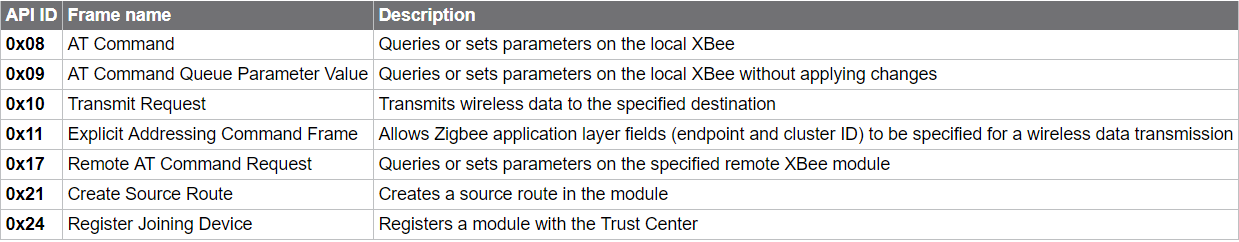
\includegraphics[width=0.9\textwidth]{figuras/txAPIFrames.png}
\caption{API Frames de transmisión}
\label{fig:txAPI}
\end{figure}

\begin{figure}[H]
\centering
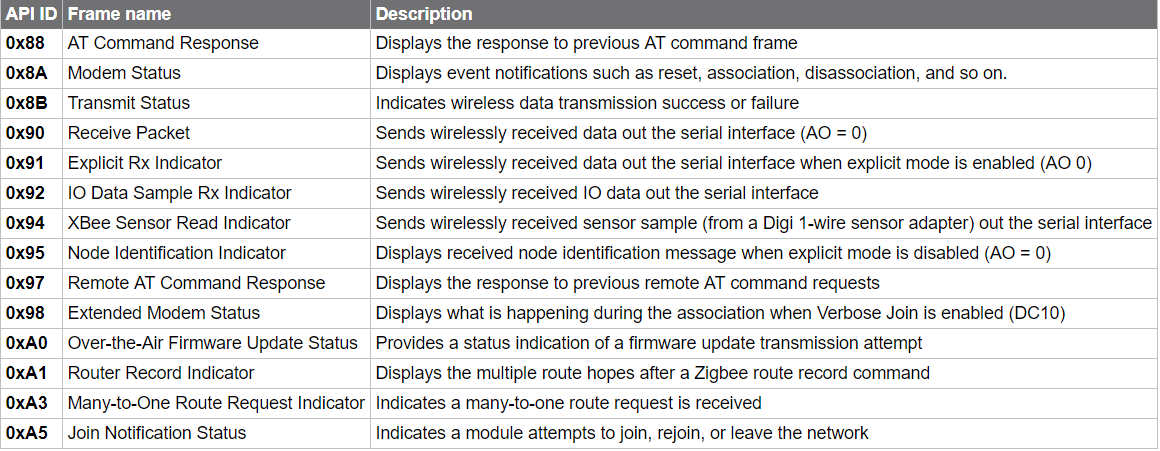
\includegraphics[width=0.9\textwidth]{figuras/rxAPIFrames.png}
\caption{API Frames de recepción}
\label{fig:rxAPI}
\end{figure}

Para que un módulo configurado en este modo pueda emitir datos por radio, la información recibida por DIN debe adecuarse a los frames preestablecidos.

Si bien este modo aumenta la complejidad de los frames transmitidos, tiene la ventaja de contener la dirección de destino en el propio frame. Esto permite filtrar los receptores del mensaje en el propio mensaje, sin necesidad de acceder a la configuración del módulo XBee. Además, es posible recibir feedback de la transmisión del mensaje ya que la recepción de unos tipos de mensaje provocan la emisión de vuelta de otros que indican su recepción.

En el script sendAPI.py (apartado \ref{subsubsec:sendapi}) se genera un API frame de tipo 0x10 \textit{Transmit Request}.

\end{itemize}

\subsubsection{Funciones de los módulos}

Existen tres posibles funciones de cada módulo XBee dependiendo de la posición que que ocupen en la red domótica. Cada función de XBee implica ligeros cambios en el firmware del módulo. En la figura \ref{fig:XbeeRed} se puede observar un ejemplo de red domótica usando XBee.



\begin{itemize}
\item \textbf{Coordinador}

El coordinador es el nodo central de la red. Su presencia en la red domótica es obligatoria y única (sólo se permite un nodo coordinador en la red). Se encarga de gestionar el resto de dispositivos, conecta y desconecta dispositivos de la red, asigna direcciones, traza mandatos y gestiona el consumo de energía pudiendo dormir al resto de dispositivos. Nunca puede apagarse o ponerse en modo de ahorro de energía.

\begin{figure}[H]
\centering
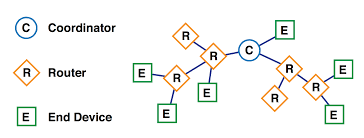
\includegraphics[width=0.9\textwidth]{figuras/XbeeRed.png}
\caption{Ejemplo de red XBee}
\label{fig:XbeeRed}
\end{figure}

En el caso del presente proyecto, se tratará del nodo unido a la Raspberry Pi, que funciona como unidad de mando.

\item \textbf{Router}

El Router es un nodo con funciones completas, puede mandar y recibir información. Puede unirse a redes existentes y se usa, principalmente, para extender la red domótica más alla del alcance del Coordinador. Se encarga de ser mensajero trasladando información desde el coordinador hasta \textit{End devices} u otros Routers; pudiendo llegar a modificar esta información.

Efectivamente, puede haber más de un router en la red y se encargan de gestionar los \textit{End devices} que tengan conectados, pudiéndoles poner en modo ahorro de energía. No pueden ponerse en modo ahorro de energía y deben estar encendidos todo el tiempo, como el coordinador

En el caso de la conexión de RHA, el XBee del brazo robótico tomará la función de router ya que precisa de una comunicación bidireccional con el Coordinador.

\item \textbf{End Device}

Los \textit{End Devices} son nodos extremos que pueden unirse a una red preexistente pero no pueden gestionar ningún dispositivo de ella. Pueden ponerse a ellos mismos en distintos modos de ahorro de energía. Las redes pueden tener un número muy alto de \textit{End Devices}, tantos como direcciones sean almacenables en el nodo coordinador.

Su uso suele estar orientado al envío de la medida de algún sensor.

\end{itemize}

\subsubsection{XCTU}\label{subsubsec:xctu}

Para configurar los módulos Xbee, Digi proporciona un software llamado XCTU\footnote{Puede descargarse desde \url{https://www.digi.com/products/iot-platform/xctu}}. 

Una vez conectado el dispositivo XBee, el primer paso es descubrirlo. Haciendo click en el icono destinado a ello, seleccionando el puerto e indicando las opciones sobre las que escanear dispositivos se iniciará la búsqueda. Sólo queda añadir el dispositivo cuando aparezca en pantalla.

Una vez añadido, se cargará la configuración actual en la interfaz de Node-RED (figura \ref{fig:XCTU} y  se podrán visualizar y modificar todos los parámetros.

\begin{figure}[tb]
\centering
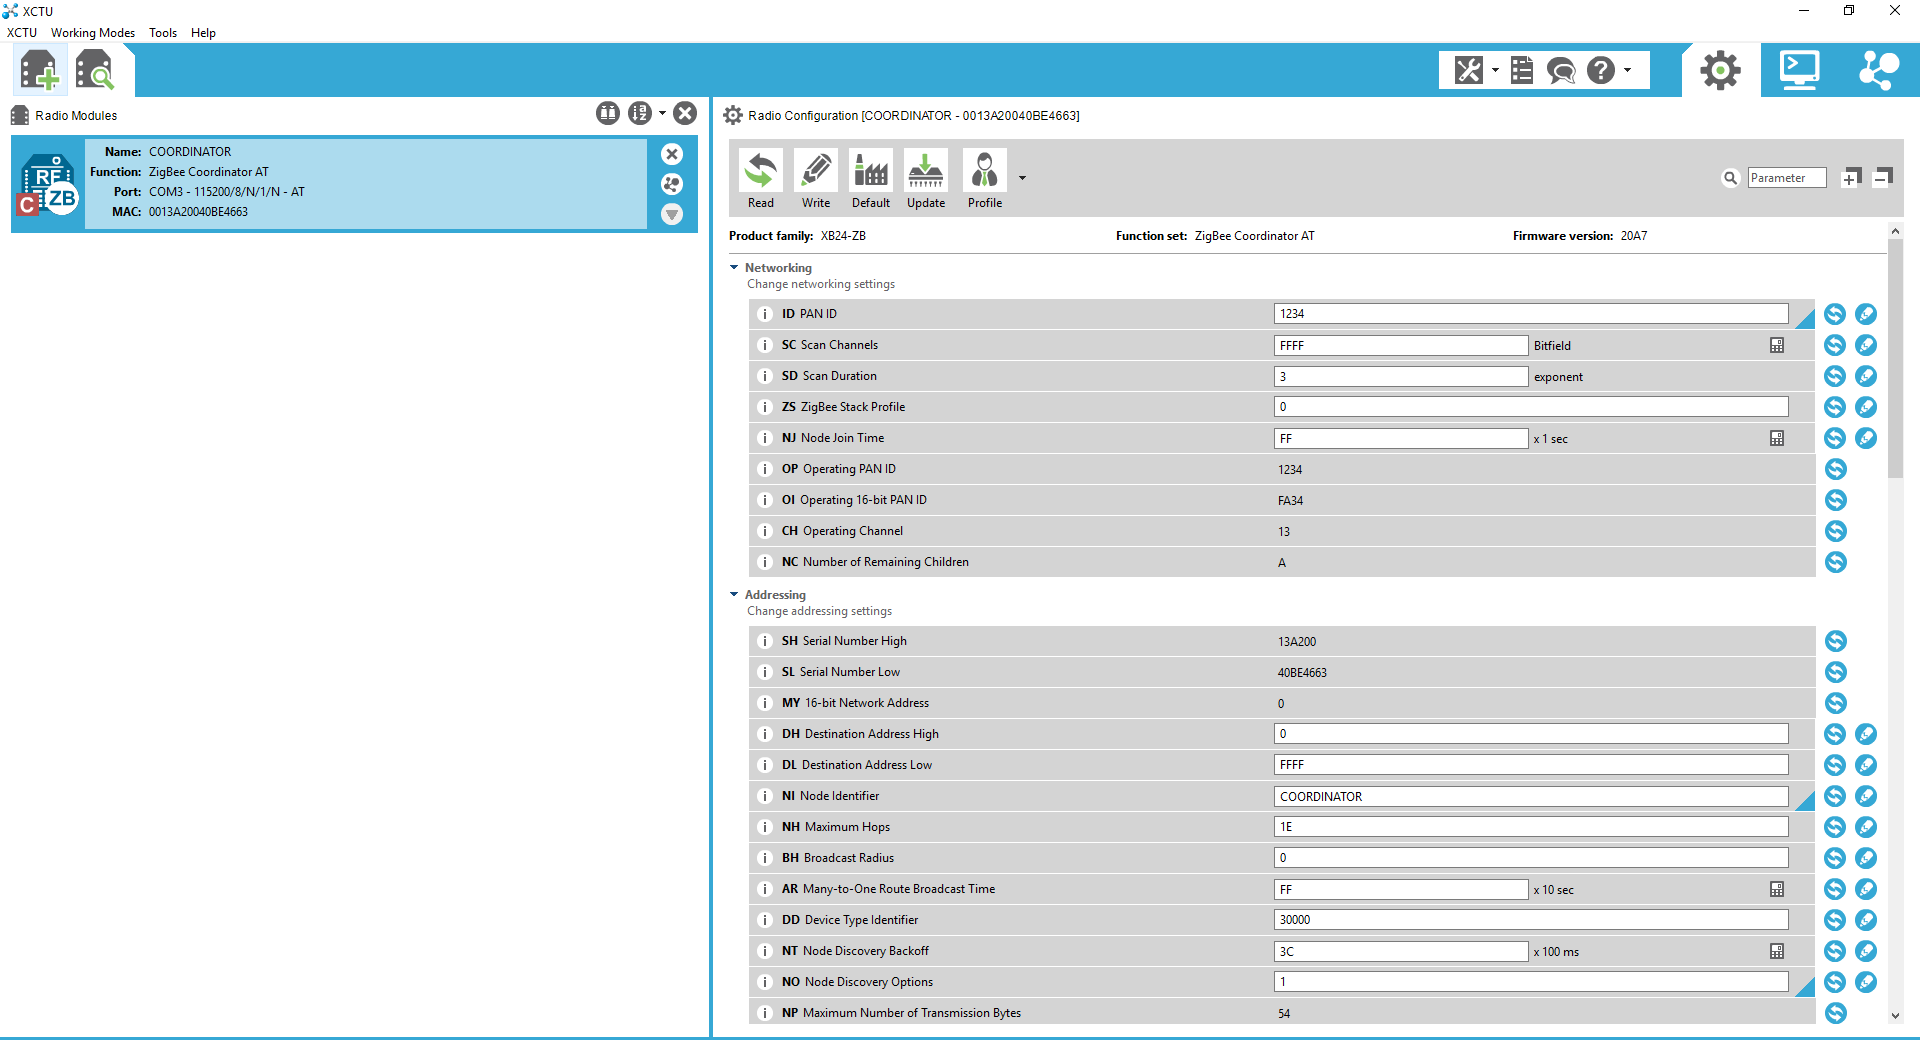
\includegraphics[width=0.9\textwidth, frame]{figuras/interfazXCTU.png}
\caption{Iterfaz de XCTU}
\label{fig:XCTU}
\end{figure}

Para cambiar el firmware, se puede hacer click en \textit{Update} (figura \ref{fig:firmXCTU}) y seleccionar un nuevo firmware y versión. Es en esta pantalla en la que se puede cargar firmware orientado a un modo de comunicación en concreto (AT o API). Al hacer click en Update comenzará el proceso de escritura del firmware y, tras unos segundos, el módulo estará listo para usarse. 

\begin{figure}[h]
\centering
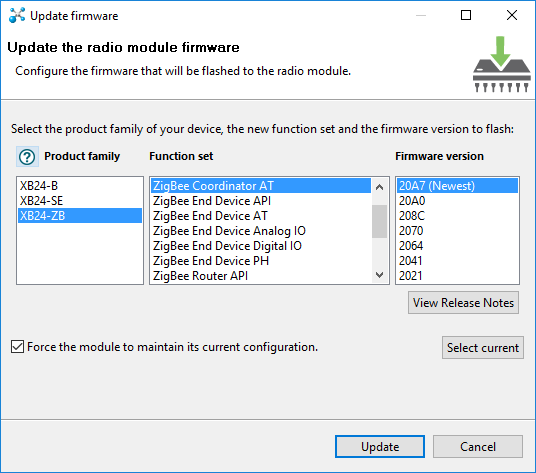
\includegraphics[width=0.5\textwidth]{figuras/firmXCTU.png}
\caption{Carga de firmware en XCTU}
\label{fig:firmXCTU}
\end{figure}

La interfaz de XCTU permite modificar multitud de parámetros que deben coincidir en todos los extremos de la comunicación. En la figura \ref{fig:XCTUPropCoord} se pueden observar los parámetros de configuración del XBee Coordinador AT, mientras que en la figura \ref{fig:XCTUPropRou} está la configuración del Router AT. En modo API son similares

\begin{figure}[H]
\centering
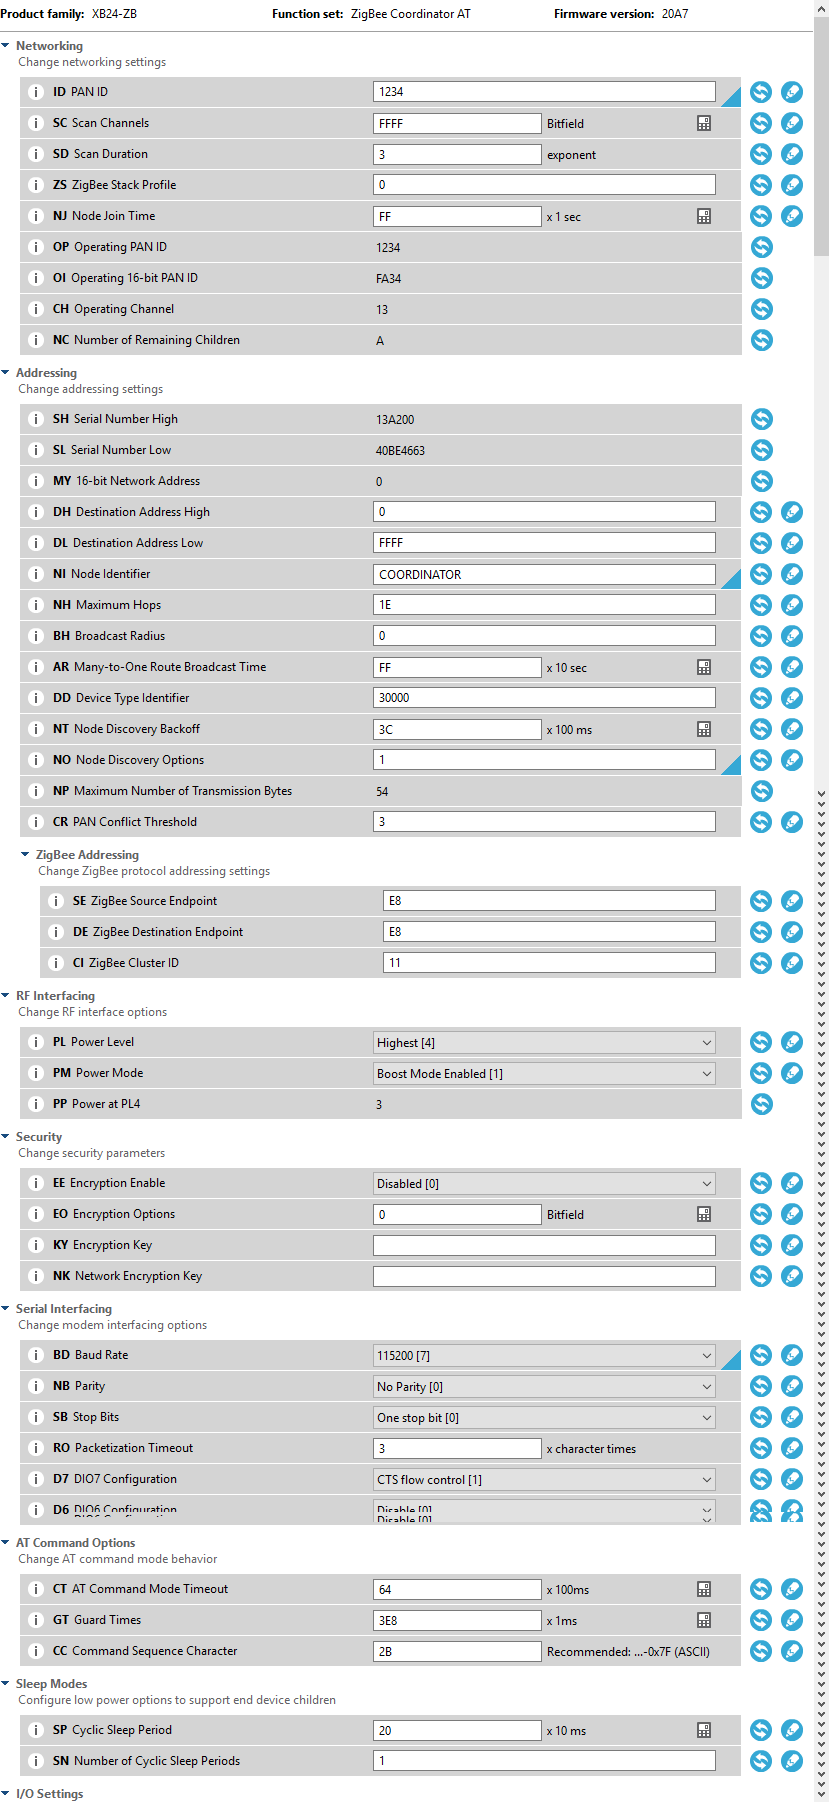
\includegraphics[width=0.75\textwidth]{figuras/XCTUPropCoord.png}
\caption{Propiedades del XBee Coordinador AT}
\label{fig:XCTUPropCoord}
\end{figure}

\begin{figure}[H]
\centering
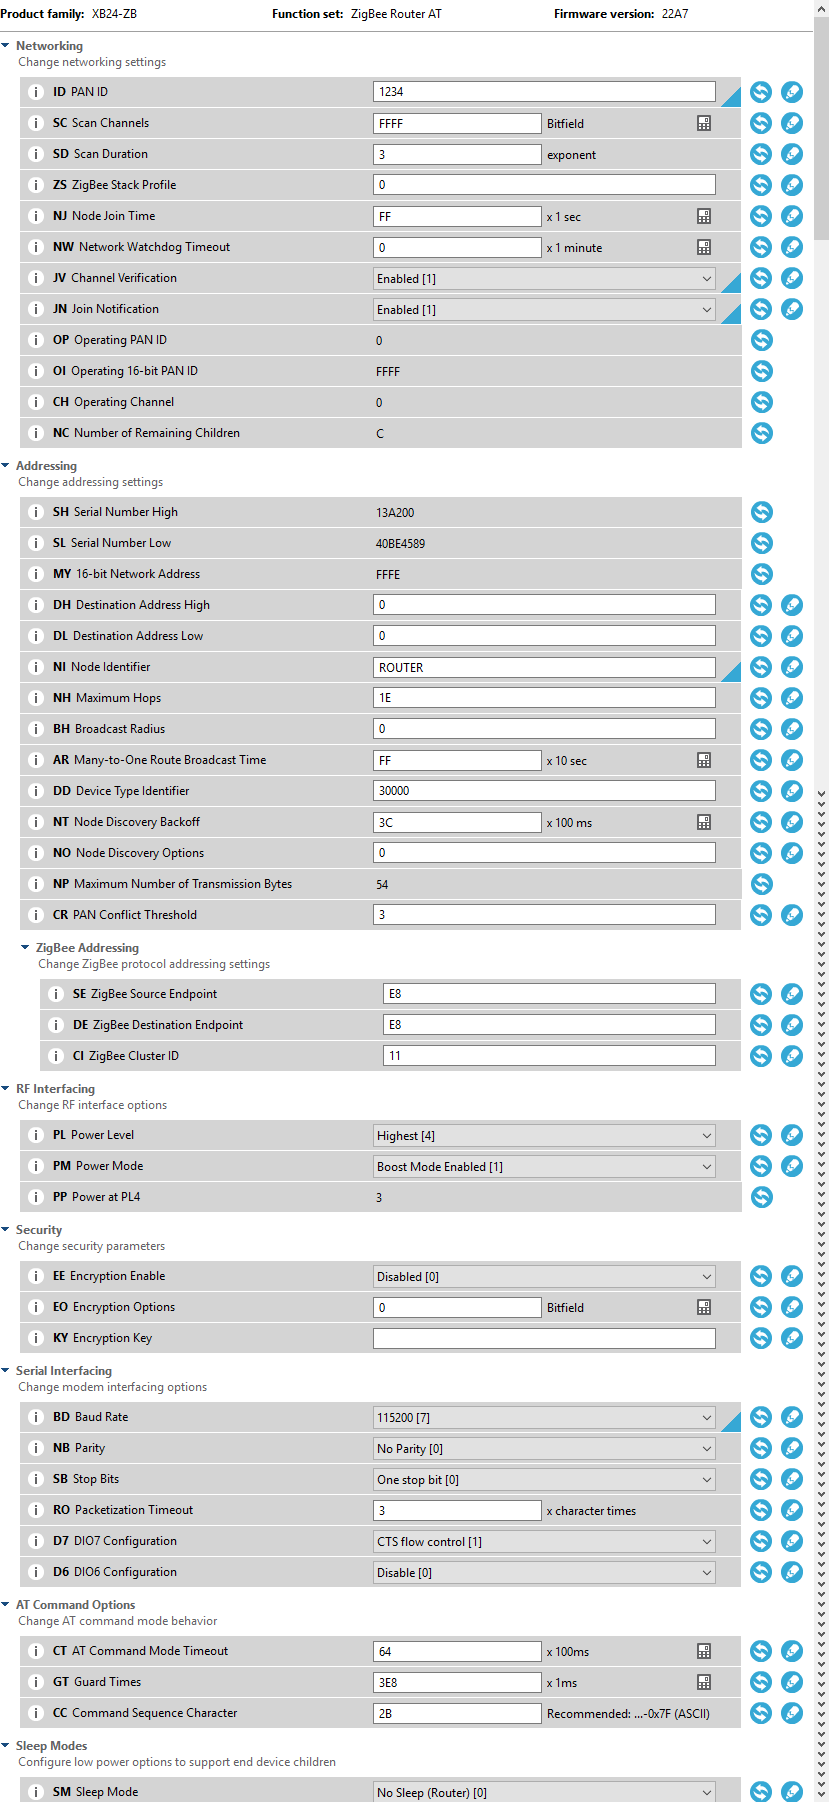
\includegraphics[width=0.75\textwidth]{figuras/XCTUPropRou.png}
\caption{Propiedades del XBee Router AT}
\label{fig:XCTUPropRou}
\end{figure}

Entre los parámetros configurables más destacables se encuentran los siguientes:

\begin{itemize}
\item \textbf{PAN ID} es el identificador de la red domótica.
\item \textbf{DH} y \textbf{DL} ponen límites a las direcciones entre las cuales el dispositivo transmitirá. Estas configuraciones a 0 en el router ponen al coordinador de la red como único destinatario.
\item \textbf{NI} es el nombre identificador del nodo.
\item \textbf{EE} maneja la posibilidad de encriptar la información para añadir una capa extra de seguridad.
\item \textbf{BD}, \textbf{NB} o \textbf{SB} son los parámetros correspondientes a la comunicación serial. En este caso, se sitúa la tasa de baudios en 115200, que es el máximo admitible por XCTU.
\end{itemize}

Por último, queda comentar la posibilidad de usar XCTU como terminal serie de manera sencilla y adaptada a la aplicación que estamos comentando. En la pestaña de consolo se puede consultar la emisión y recepción de cada módulo, como se muestra en la figura \ref{fig:XCTUconsola}.

\begin{figure}[bth]
\centering
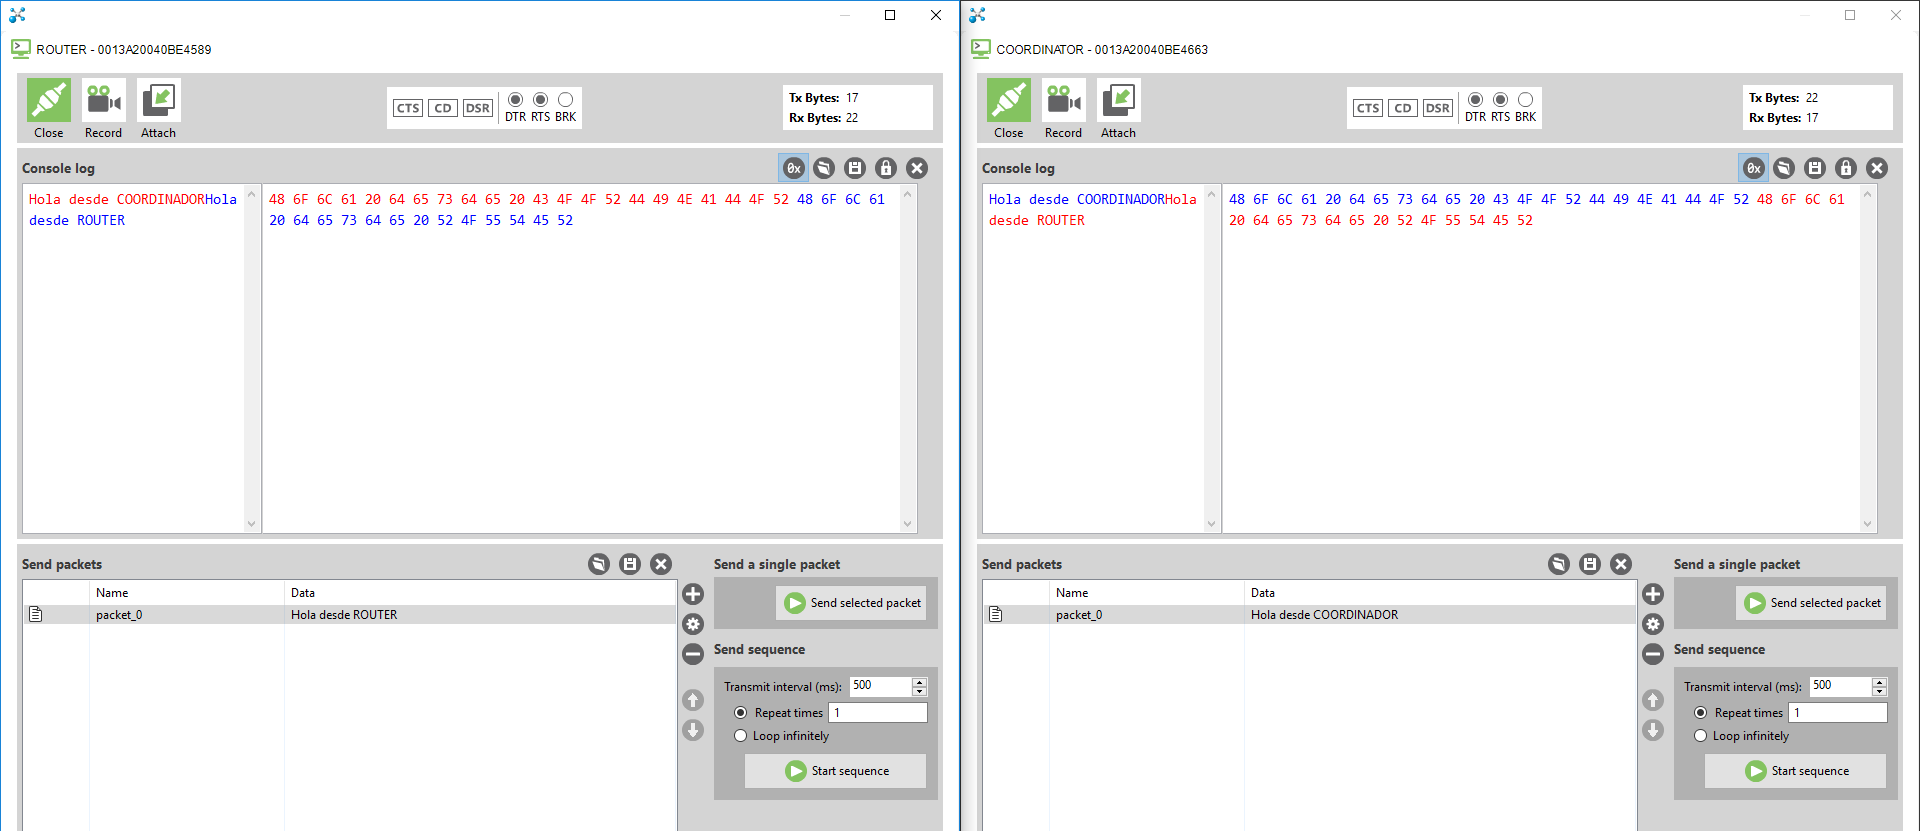
\includegraphics[width=1.1\textwidth, frame]{figuras/XCTUConsola.png}
\caption{Interfaz de consola de XCTU}
\label{fig:XCTUconsola}
\end{figure}


\subsubsection{Perfiles de comunicación}

La configuración introducida en XCTU se puede guardar y cargar de manera sencilla a través de la figura del perfil de comunicación. Estos perfiles son archivos que almacenan el firmware utilizado junto con toda la configuración específica.

Esto posibilita, como es el caso, la generación de los perfiles:

\textit{CoordinatorAPI.xpro}

\textit{RouterAPI.xpro}

\textit{CoordinatorAT.xpro}

\textit{RouterAT.xpro}

Siendo un proceso sencillo el de carga de un perfil a un módulo, es la manera más simple y rápida de cambiar el modo de comunicación de la red. No hay posibilidad de hacerlo sin cambiar el firmware.


\subsection{XBee Shield}

La XBee Shield (figura \ref{fig:XBeeSh}) es una solución que permite una interacción sencilla con los módulos XBee. Para ello, se basa en el uso de Arduino UNO (figura \ref{fig:AUno}. La XBee Shield posee un zócalo para situar el módulo XBee, está diseñada para encajar a la perfeccion sobre el Arduino UNO y esto descubre multitud de opciones.

Los diseños, layouts y planos son libres y pueden ser encontrados en internet. En el Anexo \ref{anexo:} se localiza el esquemático de la Xbee Shield.

Posee dos jumpers selectores que establecen el modo en el que debe comportarse la XBee Shield. El hecho de que haya dos es simplemente para asegurar un modo, ambos jumpers deben situarse en la misma posición para un correcto funcionamiento. La selección de estos modos configura la conexión entre la comunicación serial del módulo XBee y la comunicación serial entre el microcontrolador y el integrado USB-to-Serial de la Arduino UNO.

\subsubsection{Modo XBee}

Una de las posiciones de los jumpers es la posición XBee. En esta posición, el pin DOUT del módulo XBee se conecta al RX del microcontrolador y, por lo tanto, al TX del USB. Por otro lado, el pin DIN estaría conectado al TX del microcontrolador y, consecuentemente, al RX del USB.

Esta configuración permite que aquello que envíe el microcontrolador sea transmitido tanto por USB al ordenador como por radiofrecuencia. Sin embargo, la recepción de datos por parte del microcontrolador se realizará únicamente desde el módulo XBee, quedando inhabilitada el envío de datos por serial desde un ordenador.

Lógicamente, ya que se desea una comunicación bidireccional de datos con una Raspberry Pi, esta configuración queda descartada.

\subsubsection{Modo USB}

El otro modo alcanzable a través de los jumpers es el modo USB. Este modo consiste en la comunicación directa del pin DOUT del XBee al RX del USB y, por su parte, la conexión del pin DIN al TX del USB. 

Esto posibilita la conexión directa del módulo XBee al ordenador siempre que ningún otro dispositivo interfiera en la comunicación. Este dispositivo puede ser, perfectamente, el microcontrolador. Es esta la razón por la que es necesario retirar el microcontrolador del Arduino UNO para que funcione de manera adecuada el modo USB\footnote{De lo contrario, el Arduino UNO funcionaría de manera normal, ignorando el Modulo XBee}. Para retirar el microcontrolador, es necesario que la versión de Arduino UNO utilizada use el microcontrolador en su empaquetado de orificio pasante colocado sobre un zócalo. La versión SMD requiere desoldarlo y no termina de ser cómodo.

Puesto que en ninguno de los puntos del proyecto requerimos del preprocesamiento de los datos por un Arduino externo, el microcontrolador no aporta ninguna utilidad. Es la configuración USB, por lo tanto, la usada a lo largo del proyecto.

En concreto, hay una situacion en la que este modo adquiere especial sentido: a la hora de configurar el módulo y, en general, al usar XCTU con un módulo XBee. Se precisa una conexión directa Xbee-ordenador que la Xbee Shield en modo USB puede proporcionar.


\section{RoboHealth Arm}

RoboHealth Arm\cite{Heredia1:2018} (figura \ref{fig:RHA}) es un brazo robótico de tres grados de libertad cuyo sistema de acción se basa en un mecanismo controlado por una serie de cuerdas que son recogidas o liberadas por unos servos. Unos potenciónetros realimentan la posición de las dos articulaciones que funcionan con este mecanismo. El tercer grado de libertad, encargado de la rotación sobre su eje, no funciona de igual manera, sino que lo hace a través de un engranaje simple sin haber forma de realimentar su posición. Por lo tanto, el control de este tercer eje es absoluto.

\begin{figure}[bth]
\centering
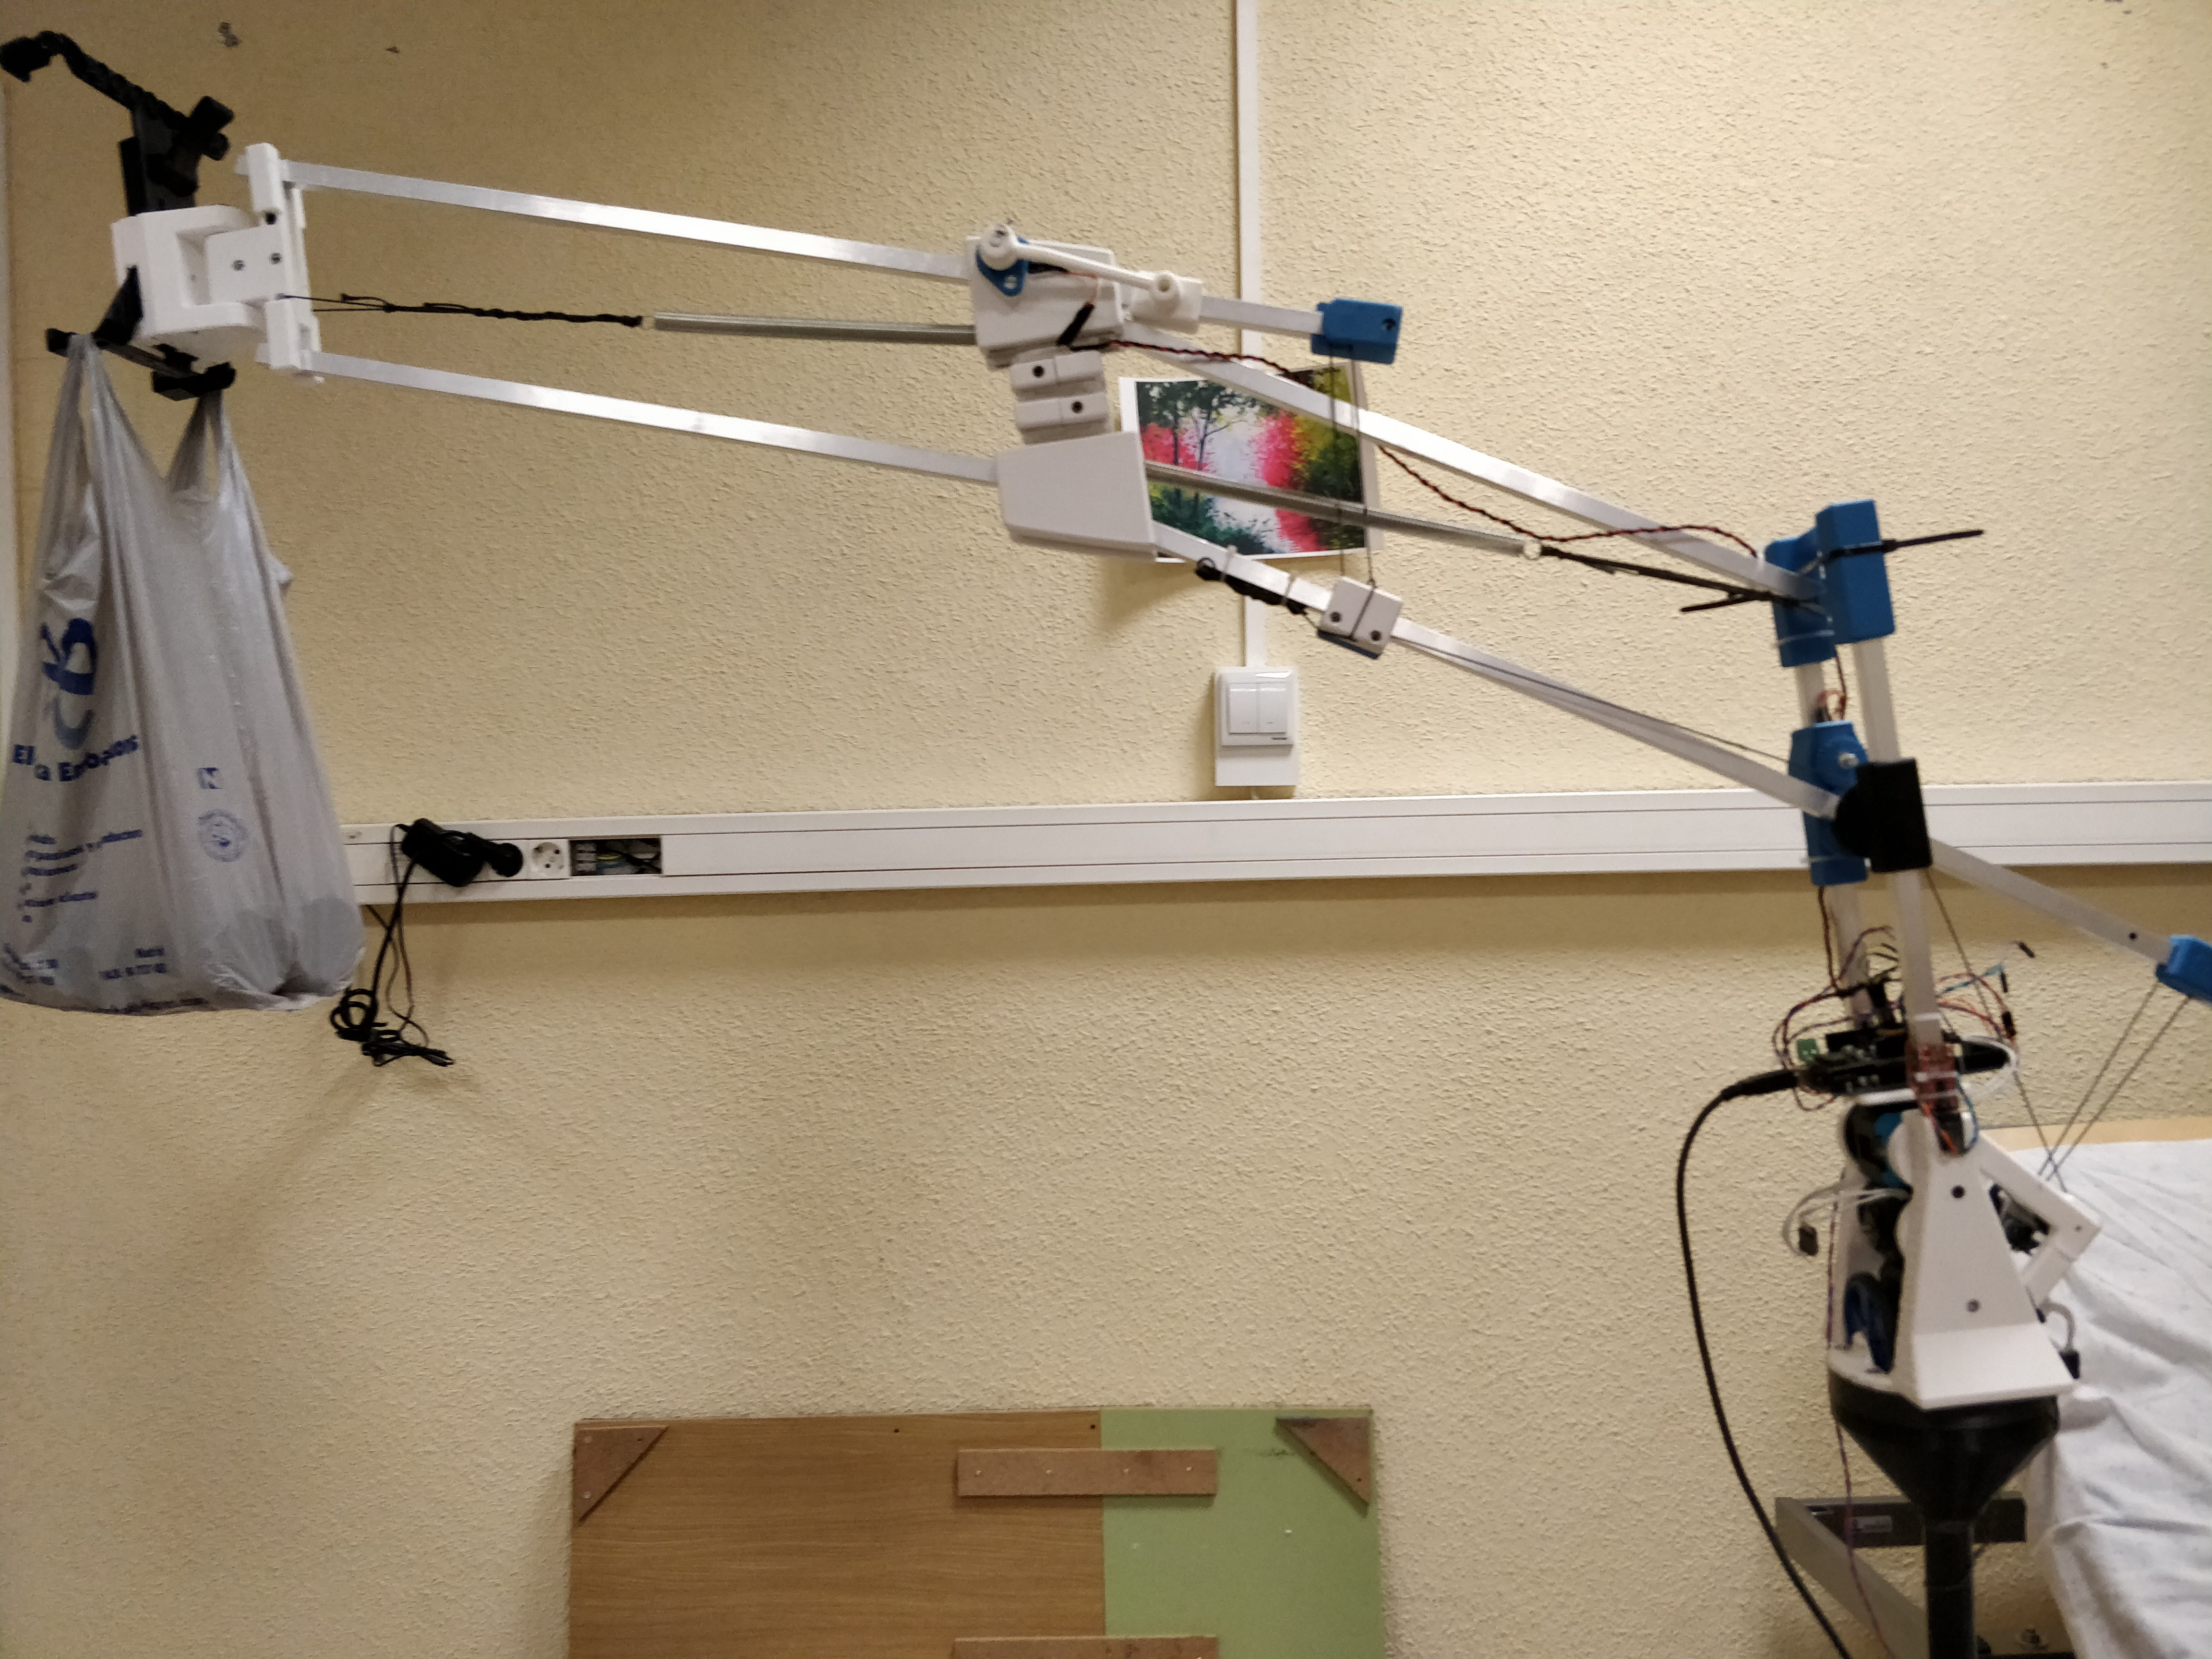
\includegraphics[width=1.1\textwidth, frame]{figuras/RHA.png}
\caption{RoboHealth Arm}
\label{fig:RHA}
\end{figure}

El programa que controla el brazo robótico\cite{Heredia2:2018} se carga sobre un microcontrolador Arduino Mega

RoboHealth Arm se trata de un Trabajo Final de Grado\cite{Heredia1:2018} realizado previamente en el marco del proyecto RoboHealth.

\subsection{Protocolo de comunicación RHA}

RoboHealth Arm incluye en su desarrollo un protocolo de comunicación detallado en \cite{Heredia1:2018}/Anexo E.

En general, este proyecto se centra en dos tipos de mensajes.

\subsection{Modificaciones a RHA}

\subsubsection{Modificaciones Hardware}

\subsubsection{Modificaciones Software}


\section{Integración}

\subsection{MQTT - Node-RED}

\begin{figure}[H]
\centering
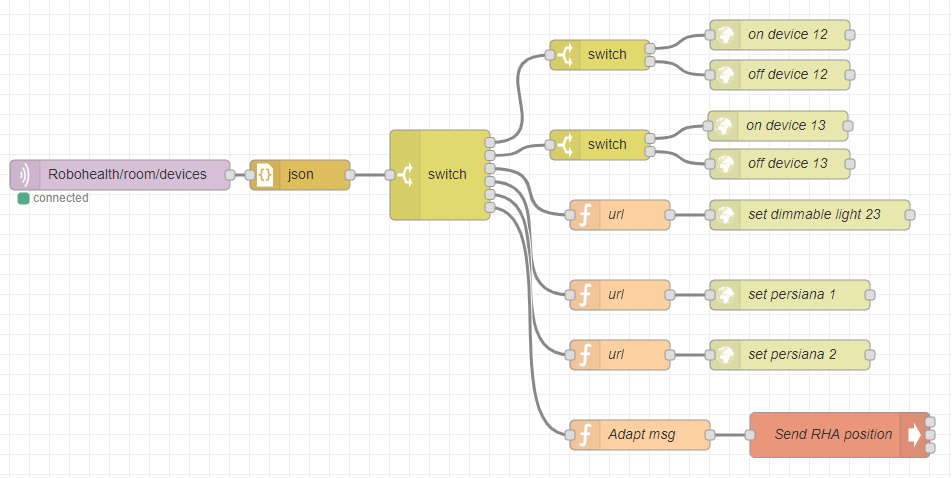
\includegraphics[width=0.9\textwidth]{figuras/MQTTFlow.png}
\caption{Flujo de recepción de MQTT}
\label{fig:MQTTFlow}
\end{figure}

\subsubsection{Flujos MQTT}

\subsection{User Interface - Node-RED}

\subsubsection{Flujos UI/Node-RED}

\subsection{Node-Red - XBee}\label{subsec:NR-Xbee}

\subsection{XBee - RHA}
